\documentclass[10pt]{article}

% Build modes: default = anonymized TMLR submission.
% For the arXiv version, compile with \def\ARXIV{1} before \input (see Makefile).
\ifdefined\ARXIV
  \usepackage[preprint]{tmlr}
  \newcommand{\codeurl}{at \url{https://github.com/maorfarid1/three-clocks}}
\else
  \usepackage{tmlr}
  \newcommand{\codeurl}{in the anonymized supplementary material}
\fi

%%%%% NEW MATH DEFINITIONS %%%%%

\usepackage{amsmath,amsfonts,bm}

% Mark sections of captions for referring to divisions of figures
\newcommand{\figleft}{{\em (Left)}}
\newcommand{\figcenter}{{\em (Center)}}
\newcommand{\figright}{{\em (Right)}}
\newcommand{\figtop}{{\em (Top)}}
\newcommand{\figbottom}{{\em (Bottom)}}
\newcommand{\captiona}{{\em (a)}}
\newcommand{\captionb}{{\em (b)}}
\newcommand{\captionc}{{\em (c)}}
\newcommand{\captiond}{{\em (d)}}

% Highlight a newly defined term
\newcommand{\newterm}[1]{{\bf #1}}


% Figure reference, lower-case.
\def\figref#1{figure~\ref{#1}}
% Figure reference, capital. For start of sentence
\def\Figref#1{Figure~\ref{#1}}
\def\twofigref#1#2{figures \ref{#1} and \ref{#2}}
\def\quadfigref#1#2#3#4{figures \ref{#1}, \ref{#2}, \ref{#3} and \ref{#4}}
% Section reference, lower-case.
\def\secref#1{section~\ref{#1}}
% Section reference, capital.
\def\Secref#1{Section~\ref{#1}}
% Reference to two sections.
\def\twosecrefs#1#2{sections \ref{#1} and \ref{#2}}
% Reference to three sections.
\def\secrefs#1#2#3{sections \ref{#1}, \ref{#2} and \ref{#3}}
% Reference to an equation, lower-case.
\def\eqref#1{equation~\ref{#1}}
% Reference to an equation, upper case
\def\Eqref#1{Equation~\ref{#1}}
% A raw reference to an equation---avoid using if possible
\def\plaineqref#1{\ref{#1}}
% Reference to a chapter, lower-case.
\def\chapref#1{chapter~\ref{#1}}
% Reference to an equation, upper case.
\def\Chapref#1{Chapter~\ref{#1}}
% Reference to a range of chapters
\def\rangechapref#1#2{chapters\ref{#1}--\ref{#2}}
% Reference to an algorithm, lower-case.
\def\algref#1{algorithm~\ref{#1}}
% Reference to an algorithm, upper case.
\def\Algref#1{Algorithm~\ref{#1}}
\def\twoalgref#1#2{algorithms \ref{#1} and \ref{#2}}
\def\Twoalgref#1#2{Algorithms \ref{#1} and \ref{#2}}
% Reference to a part, lower case
\def\partref#1{part~\ref{#1}}
% Reference to a part, upper case
\def\Partref#1{Part~\ref{#1}}
\def\twopartref#1#2{parts \ref{#1} and \ref{#2}}

\def\ceil#1{\lceil #1 \rceil}
\def\floor#1{\lfloor #1 \rfloor}
\def\1{\bm{1}}
\newcommand{\train}{\mathcal{D}}
\newcommand{\valid}{\mathcal{D_{\mathrm{valid}}}}
\newcommand{\test}{\mathcal{D_{\mathrm{test}}}}

\def\eps{{\epsilon}}


% Random variables
\def\reta{{\textnormal{$\eta$}}}
\def\ra{{\textnormal{a}}}
\def\rb{{\textnormal{b}}}
\def\rc{{\textnormal{c}}}
\def\rd{{\textnormal{d}}}
\def\re{{\textnormal{e}}}
\def\rf{{\textnormal{f}}}
\def\rg{{\textnormal{g}}}
\def\rh{{\textnormal{h}}}
\def\ri{{\textnormal{i}}}
\def\rj{{\textnormal{j}}}
\def\rk{{\textnormal{k}}}
\def\rl{{\textnormal{l}}}
% rm is already a command, just don't name any random variables m
\def\rn{{\textnormal{n}}}
\def\ro{{\textnormal{o}}}
\def\rp{{\textnormal{p}}}
\def\rq{{\textnormal{q}}}
\def\rr{{\textnormal{r}}}
\def\rs{{\textnormal{s}}}
\def\rt{{\textnormal{t}}}
\def\ru{{\textnormal{u}}}
\def\rv{{\textnormal{v}}}
\def\rw{{\textnormal{w}}}
\def\rx{{\textnormal{x}}}
\def\ry{{\textnormal{y}}}
\def\rz{{\textnormal{z}}}

% Random vectors
\def\rvepsilon{{\mathbf{\epsilon}}}
\def\rvtheta{{\mathbf{\theta}}}
\def\rva{{\mathbf{a}}}
\def\rvb{{\mathbf{b}}}
\def\rvc{{\mathbf{c}}}
\def\rvd{{\mathbf{d}}}
\def\rve{{\mathbf{e}}}
\def\rvf{{\mathbf{f}}}
\def\rvg{{\mathbf{g}}}
\def\rvh{{\mathbf{h}}}
\def\rvu{{\mathbf{i}}}
\def\rvj{{\mathbf{j}}}
\def\rvk{{\mathbf{k}}}
\def\rvl{{\mathbf{l}}}
\def\rvm{{\mathbf{m}}}
\def\rvn{{\mathbf{n}}}
\def\rvo{{\mathbf{o}}}
\def\rvp{{\mathbf{p}}}
\def\rvq{{\mathbf{q}}}
\def\rvr{{\mathbf{r}}}
\def\rvs{{\mathbf{s}}}
\def\rvt{{\mathbf{t}}}
\def\rvu{{\mathbf{u}}}
\def\rvv{{\mathbf{v}}}
\def\rvw{{\mathbf{w}}}
\def\rvx{{\mathbf{x}}}
\def\rvy{{\mathbf{y}}}
\def\rvz{{\mathbf{z}}}

% Elements of random vectors
\def\erva{{\textnormal{a}}}
\def\ervb{{\textnormal{b}}}
\def\ervc{{\textnormal{c}}}
\def\ervd{{\textnormal{d}}}
\def\erve{{\textnormal{e}}}
\def\ervf{{\textnormal{f}}}
\def\ervg{{\textnormal{g}}}
\def\ervh{{\textnormal{h}}}
\def\ervi{{\textnormal{i}}}
\def\ervj{{\textnormal{j}}}
\def\ervk{{\textnormal{k}}}
\def\ervl{{\textnormal{l}}}
\def\ervm{{\textnormal{m}}}
\def\ervn{{\textnormal{n}}}
\def\ervo{{\textnormal{o}}}
\def\ervp{{\textnormal{p}}}
\def\ervq{{\textnormal{q}}}
\def\ervr{{\textnormal{r}}}
\def\ervs{{\textnormal{s}}}
\def\ervt{{\textnormal{t}}}
\def\ervu{{\textnormal{u}}}
\def\ervv{{\textnormal{v}}}
\def\ervw{{\textnormal{w}}}
\def\ervx{{\textnormal{x}}}
\def\ervy{{\textnormal{y}}}
\def\ervz{{\textnormal{z}}}

% Random matrices
\def\rmA{{\mathbf{A}}}
\def\rmB{{\mathbf{B}}}
\def\rmC{{\mathbf{C}}}
\def\rmD{{\mathbf{D}}}
\def\rmE{{\mathbf{E}}}
\def\rmF{{\mathbf{F}}}
\def\rmG{{\mathbf{G}}}
\def\rmH{{\mathbf{H}}}
\def\rmI{{\mathbf{I}}}
\def\rmJ{{\mathbf{J}}}
\def\rmK{{\mathbf{K}}}
\def\rmL{{\mathbf{L}}}
\def\rmM{{\mathbf{M}}}
\def\rmN{{\mathbf{N}}}
\def\rmO{{\mathbf{O}}}
\def\rmP{{\mathbf{P}}}
\def\rmQ{{\mathbf{Q}}}
\def\rmR{{\mathbf{R}}}
\def\rmS{{\mathbf{S}}}
\def\rmT{{\mathbf{T}}}
\def\rmU{{\mathbf{U}}}
\def\rmV{{\mathbf{V}}}
\def\rmW{{\mathbf{W}}}
\def\rmX{{\mathbf{X}}}
\def\rmY{{\mathbf{Y}}}
\def\rmZ{{\mathbf{Z}}}

% Elements of random matrices
\def\ermA{{\textnormal{A}}}
\def\ermB{{\textnormal{B}}}
\def\ermC{{\textnormal{C}}}
\def\ermD{{\textnormal{D}}}
\def\ermE{{\textnormal{E}}}
\def\ermF{{\textnormal{F}}}
\def\ermG{{\textnormal{G}}}
\def\ermH{{\textnormal{H}}}
\def\ermI{{\textnormal{I}}}
\def\ermJ{{\textnormal{J}}}
\def\ermK{{\textnormal{K}}}
\def\ermL{{\textnormal{L}}}
\def\ermM{{\textnormal{M}}}
\def\ermN{{\textnormal{N}}}
\def\ermO{{\textnormal{O}}}
\def\ermP{{\textnormal{P}}}
\def\ermQ{{\textnormal{Q}}}
\def\ermR{{\textnormal{R}}}
\def\ermS{{\textnormal{S}}}
\def\ermT{{\textnormal{T}}}
\def\ermU{{\textnormal{U}}}
\def\ermV{{\textnormal{V}}}
\def\ermW{{\textnormal{W}}}
\def\ermX{{\textnormal{X}}}
\def\ermY{{\textnormal{Y}}}
\def\ermZ{{\textnormal{Z}}}

% Vectors
\def\vzero{{\bm{0}}}
\def\vone{{\bm{1}}}
\def\vmu{{\bm{\mu}}}
\def\vtheta{{\bm{\theta}}}
\def\va{{\bm{a}}}
\def\vb{{\bm{b}}}
\def\vc{{\bm{c}}}
\def\vd{{\bm{d}}}
\def\ve{{\bm{e}}}
\def\vf{{\bm{f}}}
\def\vg{{\bm{g}}}
\def\vh{{\bm{h}}}
\def\vi{{\bm{i}}}
\def\vj{{\bm{j}}}
\def\vk{{\bm{k}}}
\def\vl{{\bm{l}}}
\def\vm{{\bm{m}}}
\def\vn{{\bm{n}}}
\def\vo{{\bm{o}}}
\def\vp{{\bm{p}}}
\def\vq{{\bm{q}}}
\def\vr{{\bm{r}}}
\def\vs{{\bm{s}}}
\def\vt{{\bm{t}}}
\def\vu{{\bm{u}}}
\def\vv{{\bm{v}}}
\def\vw{{\bm{w}}}
\def\vx{{\bm{x}}}
\def\vy{{\bm{y}}}
\def\vz{{\bm{z}}}

% Elements of vectors
\def\evalpha{{\alpha}}
\def\evbeta{{\beta}}
\def\evepsilon{{\epsilon}}
\def\evlambda{{\lambda}}
\def\evomega{{\omega}}
\def\evmu{{\mu}}
\def\evpsi{{\psi}}
\def\evsigma{{\sigma}}
\def\evtheta{{\theta}}
\def\eva{{a}}
\def\evb{{b}}
\def\evc{{c}}
\def\evd{{d}}
\def\eve{{e}}
\def\evf{{f}}
\def\evg{{g}}
\def\evh{{h}}
\def\evi{{i}}
\def\evj{{j}}
\def\evk{{k}}
\def\evl{{l}}
\def\evm{{m}}
\def\evn{{n}}
\def\evo{{o}}
\def\evp{{p}}
\def\evq{{q}}
\def\evr{{r}}
\def\evs{{s}}
\def\evt{{t}}
\def\evu{{u}}
\def\evv{{v}}
\def\evw{{w}}
\def\evx{{x}}
\def\evy{{y}}
\def\evz{{z}}

% Matrix
\def\mA{{\bm{A}}}
\def\mB{{\bm{B}}}
\def\mC{{\bm{C}}}
\def\mD{{\bm{D}}}
\def\mE{{\bm{E}}}
\def\mF{{\bm{F}}}
\def\mG{{\bm{G}}}
\def\mH{{\bm{H}}}
\def\mI{{\bm{I}}}
\def\mJ{{\bm{J}}}
\def\mK{{\bm{K}}}
\def\mL{{\bm{L}}}
\def\mM{{\bm{M}}}
\def\mN{{\bm{N}}}
\def\mO{{\bm{O}}}
\def\mP{{\bm{P}}}
\def\mQ{{\bm{Q}}}
\def\mR{{\bm{R}}}
\def\mS{{\bm{S}}}
\def\mT{{\bm{T}}}
\def\mU{{\bm{U}}}
\def\mV{{\bm{V}}}
\def\mW{{\bm{W}}}
\def\mX{{\bm{X}}}
\def\mY{{\bm{Y}}}
\def\mZ{{\bm{Z}}}
\def\mBeta{{\bm{\beta}}}
\def\mPhi{{\bm{\Phi}}}
\def\mLambda{{\bm{\Lambda}}}
\def\mSigma{{\bm{\Sigma}}}

% Tensor
\DeclareMathAlphabet{\mathsfit}{\encodingdefault}{\sfdefault}{m}{sl}
\SetMathAlphabet{\mathsfit}{bold}{\encodingdefault}{\sfdefault}{bx}{n}
\newcommand{\tens}[1]{\bm{\mathsfit{#1}}}
\def\tA{{\tens{A}}}
\def\tB{{\tens{B}}}
\def\tC{{\tens{C}}}
\def\tD{{\tens{D}}}
\def\tE{{\tens{E}}}
\def\tF{{\tens{F}}}
\def\tG{{\tens{G}}}
\def\tH{{\tens{H}}}
\def\tI{{\tens{I}}}
\def\tJ{{\tens{J}}}
\def\tK{{\tens{K}}}
\def\tL{{\tens{L}}}
\def\tM{{\tens{M}}}
\def\tN{{\tens{N}}}
\def\tO{{\tens{O}}}
\def\tP{{\tens{P}}}
\def\tQ{{\tens{Q}}}
\def\tR{{\tens{R}}}
\def\tS{{\tens{S}}}
\def\tT{{\tens{T}}}
\def\tU{{\tens{U}}}
\def\tV{{\tens{V}}}
\def\tW{{\tens{W}}}
\def\tX{{\tens{X}}}
\def\tY{{\tens{Y}}}
\def\tZ{{\tens{Z}}}


% Graph
\def\gA{{\mathcal{A}}}
\def\gB{{\mathcal{B}}}
\def\gC{{\mathcal{C}}}
\def\gD{{\mathcal{D}}}
\def\gE{{\mathcal{E}}}
\def\gF{{\mathcal{F}}}
\def\gG{{\mathcal{G}}}
\def\gH{{\mathcal{H}}}
\def\gI{{\mathcal{I}}}
\def\gJ{{\mathcal{J}}}
\def\gK{{\mathcal{K}}}
\def\gL{{\mathcal{L}}}
\def\gM{{\mathcal{M}}}
\def\gN{{\mathcal{N}}}
\def\gO{{\mathcal{O}}}
\def\gP{{\mathcal{P}}}
\def\gQ{{\mathcal{Q}}}
\def\gR{{\mathcal{R}}}
\def\gS{{\mathcal{S}}}
\def\gT{{\mathcal{T}}}
\def\gU{{\mathcal{U}}}
\def\gV{{\mathcal{V}}}
\def\gW{{\mathcal{W}}}
\def\gX{{\mathcal{X}}}
\def\gY{{\mathcal{Y}}}
\def\gZ{{\mathcal{Z}}}

% Sets
\def\sA{{\mathbb{A}}}
\def\sB{{\mathbb{B}}}
\def\sC{{\mathbb{C}}}
\def\sD{{\mathbb{D}}}
% Don't use a set called E, because this would be the same as our symbol
% for expectation.
\def\sF{{\mathbb{F}}}
\def\sG{{\mathbb{G}}}
\def\sH{{\mathbb{H}}}
\def\sI{{\mathbb{I}}}
\def\sJ{{\mathbb{J}}}
\def\sK{{\mathbb{K}}}
\def\sL{{\mathbb{L}}}
\def\sM{{\mathbb{M}}}
\def\sN{{\mathbb{N}}}
\def\sO{{\mathbb{O}}}
\def\sP{{\mathbb{P}}}
\def\sQ{{\mathbb{Q}}}
\def\sR{{\mathbb{R}}}
\def\sS{{\mathbb{S}}}
\def\sT{{\mathbb{T}}}
\def\sU{{\mathbb{U}}}
\def\sV{{\mathbb{V}}}
\def\sW{{\mathbb{W}}}
\def\sX{{\mathbb{X}}}
\def\sY{{\mathbb{Y}}}
\def\sZ{{\mathbb{Z}}}

% Entries of a matrix
\def\emLambda{{\Lambda}}
\def\emA{{A}}
\def\emB{{B}}
\def\emC{{C}}
\def\emD{{D}}
\def\emE{{E}}
\def\emF{{F}}
\def\emG{{G}}
\def\emH{{H}}
\def\emI{{I}}
\def\emJ{{J}}
\def\emK{{K}}
\def\emL{{L}}
\def\emM{{M}}
\def\emN{{N}}
\def\emO{{O}}
\def\emP{{P}}
\def\emQ{{Q}}
\def\emR{{R}}
\def\emS{{S}}
\def\emT{{T}}
\def\emU{{U}}
\def\emV{{V}}
\def\emW{{W}}
\def\emX{{X}}
\def\emY{{Y}}
\def\emZ{{Z}}
\def\emSigma{{\Sigma}}

% entries of a tensor
% Same font as tensor, without \bm wrapper
\newcommand{\etens}[1]{\mathsfit{#1}}
\def\etLambda{{\etens{\Lambda}}}
\def\etA{{\etens{A}}}
\def\etB{{\etens{B}}}
\def\etC{{\etens{C}}}
\def\etD{{\etens{D}}}
\def\etE{{\etens{E}}}
\def\etF{{\etens{F}}}
\def\etG{{\etens{G}}}
\def\etH{{\etens{H}}}
\def\etI{{\etens{I}}}
\def\etJ{{\etens{J}}}
\def\etK{{\etens{K}}}
\def\etL{{\etens{L}}}
\def\etM{{\etens{M}}}
\def\etN{{\etens{N}}}
\def\etO{{\etens{O}}}
\def\etP{{\etens{P}}}
\def\etQ{{\etens{Q}}}
\def\etR{{\etens{R}}}
\def\etS{{\etens{S}}}
\def\etT{{\etens{T}}}
\def\etU{{\etens{U}}}
\def\etV{{\etens{V}}}
\def\etW{{\etens{W}}}
\def\etX{{\etens{X}}}
\def\etY{{\etens{Y}}}
\def\etZ{{\etens{Z}}}

% The true underlying data generating distribution
\newcommand{\pdata}{p_{\rm{data}}}
% The empirical distribution defined by the training set
\newcommand{\ptrain}{\hat{p}_{\rm{data}}}
\newcommand{\Ptrain}{\hat{P}_{\rm{data}}}
% The model distribution
\newcommand{\pmodel}{p_{\rm{model}}}
\newcommand{\Pmodel}{P_{\rm{model}}}
\newcommand{\ptildemodel}{\tilde{p}_{\rm{model}}}
% Stochastic autoencoder distributions
\newcommand{\pencode}{p_{\rm{encoder}}}
\newcommand{\pdecode}{p_{\rm{decoder}}}
\newcommand{\precons}{p_{\rm{reconstruct}}}

\newcommand{\laplace}{\mathrm{Laplace}} % Laplace distribution

\newcommand{\E}{\mathbb{E}}
\newcommand{\Ls}{\mathcal{L}}
\newcommand{\R}{\mathbb{R}}
\newcommand{\emp}{\tilde{p}}
\newcommand{\lr}{\alpha}
\newcommand{\reg}{\lambda}
\newcommand{\rect}{\mathrm{rectifier}}
\newcommand{\softmax}{\mathrm{softmax}}
\newcommand{\sigmoid}{\sigma}
\newcommand{\softplus}{\zeta}
\newcommand{\KL}{D_{\mathrm{KL}}}
\newcommand{\Var}{\mathrm{Var}}
\newcommand{\standarderror}{\mathrm{SE}}
\newcommand{\Cov}{\mathrm{Cov}}
% Wolfram Mathworld says $L^2$ is for function spaces and $\ell^2$ is for vectors
% But then they seem to use $L^2$ for vectors throughout the site, and so does
% wikipedia.
\newcommand{\normlzero}{L^0}
\newcommand{\normlone}{L^1}
\newcommand{\normltwo}{L^2}
\newcommand{\normlp}{L^p}
\newcommand{\normmax}{L^\infty}

\newcommand{\parents}{Pa} % See usage in notation.tex. Chosen to match Daphne's book.

\DeclareMathOperator*{\argmax}{arg\,max}
\DeclareMathOperator*{\argmin}{arg\,min}

\DeclareMathOperator{\sign}{sign}
\DeclareMathOperator{\Tr}{Tr}
\let\ab\allowbreak


\usepackage{hyperref}
\hypersetup{colorlinks=true,linkcolor=blue!50!black,citecolor=blue!50!black,urlcolor=blue!50!black}
\usepackage{url}
\usepackage{graphicx}
\usepackage{booktabs}
\usepackage{tabularx}
\usepackage{multirow}
\usepackage{array}
\usepackage{amsmath,amssymb,amsthm}
\usepackage{xcolor}
\usepackage{enumitem}
\usepackage{tikz}
\usetikzlibrary{arrows.meta,positioning,calc,fit,backgrounds,decorations.pathreplacing}

\newtheorem{proposition}{Proposition}
\newtheorem{conjecture}{Conjecture}
\theoremstyle{definition}
\newtheorem{definition}{Definition}
\theoremstyle{remark}
\newtheorem{remark}{Remark}

\newcommand{\op}[1]{\textbf{OP\,#1}}
\newcommand{\statusP}{\textsf{P}}
\newcommand{\statusM}{\textsf{M}}
\newcommand{\statusC}{\textsf{C}}
\newcommand{\na}{\textsf{?}}

\title{Large Language Models as Nonlinear Dynamical Systems:\\ The Three Clocks of Depth, Training, and Generation}

\author{\name Maor Farid \email maor@getleo.ai \\
      \addr Leo AI, Inc.\\
      50 Milk Street, Boston, MA 02109, United States}

\def\month{MM}
\def\year{YYYY}
\def\openreview{\url{https://openreview.net/forum?id=XXXX}}

\begin{document}

\maketitle

\begin{abstract}
A transformer language model is iterated in three ways: over layers, where the residual stream of each token is updated step by step; over optimizer steps, where the weights evolve under gradient descent; and over generated tokens, where the model feeds its own samples back as input. We call these the three clocks of a language model. Each clock has its own literature on clustering, edge of stability, loss spikes, grokking, repetition loops and temperature transitions, and these literatures rarely cite each other or the nonlinear dynamics they draw on. We place the three clocks in one framework of coupled maps, review about 200 papers, and condense the results into the Three-Clock Dictionary, which maps fifteen concepts from nonlinear dynamics onto each clock and marks every correspondence as proved, measured or conjectured. Experiments on open models, all run on a laptop CPU, put these tools to work. Training makes each layer of a Pythia model stretch perturbations more strongly, while the forward pass as a whole changes little. At the edge of stability of a small transformer, two to six Hessian eigenvalues exceed $2/\eta$ while the curvature along the step stays at $2/\eta$. Escape from repetition loops in GPT-2 and Pythia follows the Arrhenius law of Kramers' escape problem, with the logit gap as the barrier (correlation 0.997 between fitted and measured barriers), and the barrier deepens while the model repeats itself and then saturates. A loop therefore never locks for good, but the temperature needed to leave it within a budget of $N$ cycles falls like $1/\ln N$, and it rises with model size, by about half from 70M to 1B parameters. Coherent text occupies a narrow window of temperatures between repetition and incoherence. A small reasoning model, Qwen3-0.6B on grade-school math, shows the same window, with the best accuracy at the temperature its developers recommend, but at low temperature it rethinks the same step again and again without entering an exact loop. We close with twelve open problems and release code, data and a maintained reading list.

\end{abstract}

\section{Introduction}
\label{sec:intro}

\begin{figure}[t]
\centering
\begin{tikzpicture}[
  font=\small,
  layer/.style={draw=black!70, fill=blue!8, rounded corners=1.5pt, minimum width=2.3cm, minimum height=0.42cm, inner sep=1pt, font=\scriptsize},
  mini/.style={draw=black!60, fill=green!10, rounded corners=1pt, minimum width=0.85cm, minimum height=0.2cm, inner sep=0pt},
  tokbox/.style={draw=black!60, fill=orange!12, rounded corners=1pt, minimum width=0.62cm, minimum height=0.42cm, inner sep=1pt, font=\scriptsize},
  clock/.style={-{Latex[length=2.4mm]}, line width=1.1pt},
  thin/.style={-{Latex[length=1.5mm]}, black!55},
  note/.style={font=\scriptsize, align=left},
  ttl/.style={font=\small\bfseries, align=left}
]
% ================= Clock 2: training snapshots =================
\foreach \k/\x/\lab/\op in {0/-7.2/{$\theta_0$}/0.35, 1/-6.0/{$\theta_t$}/0.65, 2/-4.8/{$\theta_{\mathrm{end}}$}/1.0} {
  \begin{scope}[opacity=\op]
    \foreach \i in {0,...,5} { \node[mini] at (\x, 0.42+0.27*\i) {}; }
  \end{scope}
  \node[font=\scriptsize] at (\x, 0.05) {\lab};
}
\draw[clock, green!45!black] (-7.75, -0.3) -- (-4.25, -0.3);
\node[ttl, text=green!40!black, anchor=north west] at (-7.8, -0.45) {Clock 2: training time $t$};
\node[note, anchor=north west, text width=4.0cm] at (-7.8, -0.95) {$\theta_{t+1} = \theta_t - \eta\, g_t(\theta_t)$\\[1pt]edge of stability, catapults and loss spikes, saddle plateaus, grokking};
\draw[thin, dashed] (-4.25, 1.1) -- node[above, font=\scriptsize] {weights $\theta$} (-1.3, 1.1);

% ================= Clock 1: depth =================
\foreach \i/\lab in {0/{embed $x^{0}$}, 1/{block $\ell=1$}, 2/{block $\ell=2$}, 3/{$\cdots$}, 4/{block $\ell=L$}} {
  \node[layer] (L\i) at (0, 0.55*\i) {\lab};
}
\node[draw=black!70, fill=gray!12, rounded corners=1.5pt, minimum width=2.3cm, minimum height=0.42cm, inner sep=1pt, font=\scriptsize] (head) at (0, 2.95) {$\mathrm{softmax}(z/T)$};
\draw[thin] (L4.north) -- (head.south);
\draw[clock, blue!70!black] (1.45, -0.2) -- (1.45, 2.45);
\node[ttl, text=blue!60!black, anchor=north west] at (1.65, 2.55) {Clock 1: layer time $\ell$};
\node[note, anchor=north west, text width=3.9cm] at (1.65, 2.05) {$x^{\ell+1}_i = x^{\ell}_i + f_{\theta}^{\ell}\big(x^{\ell}_i;\, x^{\ell}_{1:n}\big)$\\[1pt]tokens as interacting particles; clustering, rank collapse, order to chaos, dynamical isometry};

% ================= Clock 3: generation =================
\foreach \j/\t in {0/{$y_1$}, 1/{$y_2$}, 2/{$\cdots$}, 3/{$y_{n}$}} {
  \node[tokbox] (T\j) at (-1.05+0.7*\j, -1.0) {\t};
}
\node[tokbox, fill=orange!40] (Tn) at (1.85, -1.0) {$y_{n+1}$};
\draw[thin] (0, -0.77) -- (L0.south);
\draw[clock, orange!80!black, rounded corners=8pt] (head.east) -- (6.0, 2.95) -- (6.0, -1.0) -- (Tn.east);
\node[ttl, text=orange!70!black, anchor=north west] at (-1.4, -1.4) {Clock 3: generation time $n$};
\node[note, anchor=north west, text width=7.2cm] at (-1.4, -1.9) {$y_{n+1} \sim \mathrm{softmax}\big(z(y_{1:n};\theta)/T\big)$: repetition loops as attractors, temperature transitions, drift, collapse};
\end{tikzpicture}
\caption{The three clocks of a transformer language model. \textbf{Clock 1} (blue) iterates the residual update over layers for a fixed input and fixed weights. \textbf{Clock 2} (green) iterates the optimizer over the weights; it hands its current weights to the model. \textbf{Clock 3} (orange) iterates sampling: each new token is appended to the context and the whole stack runs again. One tick of clock~3 contains a full run of clock~1, and clock~2 changes the map that both of them iterate. Typical behavior studied on each clock is listed next to it; Table~\ref{tab:dictionary} maps it onto dynamical-systems concepts.}
\label{fig:clocks}
\end{figure}


A transformer language model is a nonlinear map. It takes a context, a sequence of tokens, and returns a probability distribution over the next token, much as a forced pendulum maps an initial condition and an excitation to a history of displacements.\footnote{Use of AI tools: an AI assistant (Claude, Anthropic) helped search and verify the literature, draft and edit text, and write and run the experiment code, under the author's direction. All references were checked against arXiv or Crossref records and all reported numbers come from the released code. The author takes full responsibility for the content.} The analogy has one important limit. In a mechanical model the parameters, such as the length of a pendulum or the stiffness of a frame under earthquake loading, are fixed or prescribed from outside, whereas a learning model changes its own parameters, and it does so through a second dynamical system, the training algorithm. A language model is therefore used as an iterated map in at least three different ways, and each of these iterations has its own literature, its own vocabulary and its own catalogue of strange behavior.

The first iteration runs over depth. Each residual block adds an update to the hidden state of every token, so a stack of $L$ blocks is a discrete-time dynamical system with the layer index as time \citep{e2017proposal,haber2017stable,lu2017finite,chen2018neural}, and attention couples the tokens into a system of interacting particles \citep{lu2019improving,sander2021sinkformers,geshkovski2023mathematical}. The second iteration runs over optimization steps. Gradient descent is a map on parameter space, and at the step sizes used in practice it sits at the boundary of linear stability \citep{cohen2021gradient}, produces loss spikes \citep{chowdhery2022palm,wortsman2023smallscale} and goes through abrupt transitions such as grokking \citep{power2022grokking} and the formation of induction heads \citep{olsson2022incontext}. The third iteration runs over generated tokens. An autoregressive model feeds its own samples back as input, so decoding is a stochastic dynamical system on the space of contexts, and its best known pathology, the repetition loop \citep{holtzman2019curious,xu2022learning}, has recently been analyzed as an attractor \citep{wang2025unveiling,jones2026chaos}.

We call these three iterations the \emph{three clocks} of a language model, with layer time $\ell$, training time $t$ and generation time $n$ (Figure~\ref{fig:clocks}). The clocks are coupled, since the parameters produced by clock~2 define the map iterated by clock~1, and every tick of clock~3 calls a full run of clock~1. They also run at very different rates, since the weights do not move during generation and each weight update in training averages over many forward passes. Separated time scales of this kind are the standard setting of slow-fast dynamical systems \citep{strogatz2018nonlinear}, and they explain why three literatures could grow up around one object with few citations between them.

The cost of this separation is that well-understood dynamics is rediscovered under new names. Nonlinear dynamics has a mature theory for the behaviors that appear on the three clocks, built over more than a century on pendulums, rotating machinery, ships, lasers and networks of coupled oscillators: stability and bifurcations, synchronization, chaos and Lyapunov exponents, and noise-driven escape from potential wells \citep{strogatz2018nonlinear,kramers1940brownian,hanggi1990reaction,acebron2005kuramoto}. These tools transfer directly. Escape from a repetition loop at sampling temperature $T$ is the escape of a particle from a potential well under noise of intensity $T$, with the gap between the logits of the repeated token and its best competitor in the role of the barrier. The Arrhenius form of the Kramers rate then predicts how the escape probability depends on temperature, and the measured growth of the barrier predicts how long a loop survives (Section~\ref{sec:loops} and Experiment~3). The exchange also runs the other way. Neural networks already forecast spatiotemporally chaotic systems from data \citep{pathak2018model} and learn coordinates in which nonlinear dynamics becomes linear \citep{lusch2017deep}, and a trained transformer is itself a high-dimensional, nonautonomous system that can be run millions of times, observed completely and differentiated exactly.

A bridge between two fields can carry three kinds of traffic. The first is description, in which a behavior seen in one field receives a model, a name and a set of measurable quantities from the other, so that a repetition loop becomes a periodic orbit and a step-to-step oscillation of the loss becomes a period-2 orbit of a map. The second is explanation, in which the tools of the older field account for why the behavior occurs and predict how it changes with a parameter, as Kramers' theory predicts how the rate of escape from a well changes with the noise. The third is solution, in which the explanation points to an intervention that fixes a problem the newer field had not solved. Most of this paper works at the first two levels. Figures~\ref{fig:pair_training} to~\ref{fig:pair_depth} show the description directly, with a mechanical system and a language model drawn in the same representation, and Section~\ref{sec:reduced} explains each correspondence with a reduced-order model, in the way an engineer replaces a sloshing tank or a rolling ship by an equivalent oscillator. The softmax turns out to be a Boltzmann distribution, gradient descent an Euler step on a nonlinear spring, attention on the circle a Kuramoto model, and a repetition loop a well that deepens while it is occupied. At the third level we tested three controllers derived from the escape analysis on GPT-2. They remove exact loops and find the temperature window without a sweep, but none produces more coherent text than the best fixed temperature, because the trap is stored in the context while the controllers act on the noise (\op{12}). Solutions at this level remain the main open task, and the open problems of Section~\ref{sec:open} list the places where we expect them.

In the current work we build this bridge in both directions. We write the three clocks in the language of nonlinear dynamics, record which correspondences are proved, measured or only conjectured, and use the tools of the field to explain behavior that the machine learning literature documents but does not yet explain. Our contributions are the following.
\begin{enumerate}[leftmargin=*,itemsep=2pt]
\item \textbf{A unified framework.} We formalize the three clocks as coupled maps, show textbook physical systems and language models side by side, and derive the reduced-order models behind each correspondence (Section~\ref{sec:primer}) and review the dynamical-systems results for each clock (Sections~\ref{sec:clock1}, \ref{sec:clock2} and~\ref{sec:clock3}), drawing on about 200 papers from machine learning theory, interpretability, optimization, statistical physics and applied mathematics.
\item \textbf{The Three-Clock Dictionary.} Table~\ref{tab:dictionary} maps fifteen concepts from nonlinear dynamics (fixed points, limit cycles, period doubling, Lyapunov exponents, basins, metastability, noise-driven escape, synchronization, Koopman linearization and others) onto observed behavior on each clock, with the evidence level of every entry. An empty cell marks a concept that no study we found has tested on that clock, and each such cell defines a research question.
\item \textbf{Experiments} on open models that run on a laptop CPU (Section~\ref{sec:experiments}). We measure how the per-layer Lyapunov profile of the residual stream changes over training in the public Pythia checkpoints \citep{biderman2023pythia}, we compute a learning-rate bifurcation diagram of a small transformer trained by full-batch gradient descent and show that at the edge of stability several Hessian eigenvalues exceed $2/\eta$ while the curvature along the step stays at $2/\eta$, and we show that escape from repetition loops in GPT-2 and Pythia follows an Arrhenius law with the logit gap as the Kramers barrier \citep{kramers1940brownian}, a barrier that grows while the model stays in the loop and then saturates. We prove that logarithmic growth would give a sharp locking temperature, show that the measured growth saturates instead, so that the locking temperature falls with the length of the generation and rises with model size from 70M to 1B parameters, and map the narrow window of temperatures between repetitive and incoherent text. In a small reasoning model the same window appears, centered on the temperature its developers recommend, but its lower edge is set by recurrent rethinking, and no exact loop forms.
\item \textbf{Twelve open problems} (Section~\ref{sec:open}), each stated with a first test.
\end{enumerate}

Several papers develop one of these views in depth, and we rely on them throughout. \citet{geshkovski2023mathematical} and \citet{castin2025unified} develop the mathematics of attention as an interacting particle system over depth. \citet{cohen2021gradient} and the work that followed analyze gradient descent at the edge of stability. \citet{krishnamurthy2026stochastic} give a stochastic dynamical-systems account of autoregressive generation and of networks of interacting language models, and \citet{jones2026chaos} studies chaos and bifurcations in a deterministic feedback version of generation. To our knowledge, no earlier work treats the three clocks side by side in one vocabulary, with an explicit record of which correspondences are proved, which are measured and which are conjectures.

We use the language of dynamical systems in its technical sense wherever a result supports it, and we flag analogies as analogies. For example, we call a loss spike a bifurcation only when a parameter can be shown to cross a stability threshold. The paper is written for machine learning researchers who want a compact entry into dynamical-systems tools, and for dynamicists who want to know which of their tools are already in use on language models. Section~\ref{sec:primer} is a primer for the first group, and the dictionary in Section~\ref{sec:dictionary} is intended for both.

\begin{center}
\fbox{\begin{minipage}{0.94\linewidth}
\textbf{Practical takeaways.}
\begin{itemize}[leftmargin=*,itemsep=1pt,topsep=2pt]
\item \emph{Generation.} In GPT-2 and Pythia, coherent text appears only in a narrow band of temperatures between repetition and incoherence, and for some prompts in none. A loop is not locked by a fixed temperature: the temperature needed to leave it within a given budget falls like $1/\ln N$ with the length $N$ of the generation, and larger models need a higher temperature to leave the same kind of loop (Section~\ref{sec:exp3}). In Qwen3-0.6B on GSM8K, accuracy within a fixed budget peaks at the vendor's $T=0.6$, and below it the model rethinks the same step until the budget runs out.
\item \emph{Anti-repetition.} Raising the temperature when a loop starts, rolling the text back to the start of the loop, or steering the temperature by feedback all remove exact loops, but none beats the best fixed temperature on coherent text, because the attractor is stored in the context, not in the sampler (\op{12}).
\item \emph{Training.} At the edge of stability several Hessian eigenvalues sit 5\% to 14\% above $2/\eta$ while the curvature along the actual step equals $2/\eta$, so $\eta\lambda_{\max}>2$ alone does not signal divergence. A power iteration can underestimate $\lambda_{\max}$ there, because the top eigenvalues form a cluster that reorders at every step (Section~\ref{sec:exp2}).
\item \emph{Depth.} Training makes each layer stretch perturbations more, while the stretched directions of consecutive layers become less aligned (Section~\ref{sec:exp1}).
\item \emph{Tools.} Per-layer Lyapunov exponents, learning-rate bifurcation diagrams and exact loop-escape probabilities from a single greedy pass all run on a laptop CPU, and the code is released.
\end{itemize}
\end{minipage}}
\end{center}


\section{The three clocks, and a primer on the tools}
\label{sec:primer}

\subsection{Three coupled maps}
\label{sec:maps}

Fix a decoder-only transformer \citep{vaswani2017attention} with $L$ residual blocks, model width $d$ and vocabulary $\mathcal{V}$. For a context of $n$ tokens, write $x^{\ell}=(x^{\ell}_1,\dots,x^{\ell}_n)\in\mathbb{R}^{n\times d}$ for the residual stream after block $\ell$, and $\theta$ for all parameters. The model defines three maps.

\begin{definition}[Clock 1: layer time]
\label{def:clock1}
For fixed $\theta$ and fixed input tokens,
\begin{equation}
x^{\ell+1} = x^{\ell} + f^{\ell}_{\theta}(x^{\ell}), \qquad \ell = 0,\dots,L-1,
\label{eq:clock1}
\end{equation}
where $f^{\ell}_\theta$ contains attention, which couples token $i$ to tokens $j\le i$, and a token-wise MLP. The logits are $z = W_U\, \mathrm{LN}(x^{L}_n)$.
\end{definition}

\begin{definition}[Clock 2: training time]
\label{def:clock2}
For a loss $\mathcal{L}$ and data stream $\xi_t$,
\begin{equation}
\theta_{t+1} = \theta_t - \eta_t\, P_t\, \nabla_\theta \ell(\theta_t;\xi_t), \qquad t = 0,1,\dots
\label{eq:clock2}
\end{equation}
where $P_t$ is a preconditioner (identity for gradient descent, a diagonal matrix built from gradient moments for Adam) and $\ell(\cdot;\xi_t)$ is the minibatch loss. With full batches the map is deterministic; with minibatches it is a random dynamical system.
\end{definition}

\begin{definition}[Clock 3: generation time]
\label{def:clock3}
For fixed $\theta$, a sampling temperature $T>0$ and a context $s_n=(y_1,\dots,y_n)$,
\begin{equation}
y_{n+1}\sim \pi_T(\cdot\mid s_n) = \mathrm{softmax}\big(z(s_n;\theta)/T\big), \qquad s_{n+1} = (s_n, y_{n+1}).
\label{eq:clock3}
\end{equation}
This is a Markov chain on the growing space of contexts. Truncation rules such as top-$k$ or nucleus sampling change $\pi_T$ but not the structure.
\end{definition}

The three maps are nested. Evaluating $z(s_n;\theta)$ in \eqref{eq:clock3} means running \eqref{eq:clock1} to the end, and computing the gradient in \eqref{eq:clock2} means running \eqref{eq:clock1} on teacher-forced contexts. The weights produced by \eqref{eq:clock2} define the maps in \eqref{eq:clock1} and \eqref{eq:clock3}. In practice the clocks also run at very different speeds relative to each other: generation never changes $\theta$, and a single training step changes the forward map only by $O(\eta)$. In the language of slow-fast systems, clock~2 is the slow variable and clocks~1 and~3 are fast dynamics evaluated at a frozen slow state \citep{strogatz2018nonlinear}. Two well-studied effects break this picture: in-context learning, where the fast clock~1 appears to run an optimizer of its own \citep{oswald2022transformers,akyurek2022learning}, and self-training on model outputs, where clock~3 feeds clock~2 \citep{shumailov2023curse,bertrand2023stability}. Both are discussed in Sections~\ref{sec:clock1} and~\ref{sec:clock3}.

\subsection{A short primer}
\label{sec:tools}

This subsection collects the dynamical-systems vocabulary used later. Readers who know it can skip to Section~\ref{sec:clock1}; a longer treatment is in \citet{strogatz2018nonlinear}.

\paragraph{Maps, fixed points and stability.} A discrete-time system is a map $u_{k+1}=F(u_k)$. A fixed point $u^\ast=F(u^\ast)$ is linearly stable if every eigenvalue of the Jacobian $DF(u^\ast)$ lies inside the unit circle. For gradient descent on a quadratic with Hessian eigenvalue $\lambda$, the map $u\mapsto(1-\eta\lambda)u$ is stable exactly when $\eta\lambda<2$. This one-line calculation is the origin of the threshold $2/\eta$ in the edge-of-stability literature (Section~\ref{sec:eos}).

\paragraph{Periodic orbits and bifurcations.} A period-$k$ orbit is a fixed point of $F^{k}$, and under a change of parameter such orbits can appear, disappear or exchange stability. A saddle-node bifurcation creates or destroys a pair of fixed points; after it, the system passes slowly through the region where they used to be (a ``ghost''), which produces long plateaus followed by fast jumps \citep{strogatz2018nonlinear,dinc2025ghost}. In a period-doubling bifurcation an eigenvalue crosses $-1$ and a period-2 orbit is born; a cascade of such doublings is a standard route to chaos.

\paragraph{Lyapunov exponents.} For a trajectory $u_0,u_1,\dots$ the finite-time Lyapunov exponent over $K$ steps is
\begin{equation}
\lambda_K(u_0) = \frac{1}{K}\log \sigma_{\max}\big(DF(u_{K-1})\cdots DF(u_0)\big),
\label{eq:ftle}
\end{equation}
where $\sigma_{\max}$ is the largest singular value. Positive values mean that nearby trajectories separate exponentially; the limit $K\to\infty$, when it exists, is the largest Lyapunov exponent. Deep networks have a fixed and small number of steps, so only finite-time exponents make sense for clock~1 \citep{storm2023finitetime}.

\paragraph{Basins and metastability.} Boundaries between basins of attraction can be fractal, as in the hyperparameter space of neural network training \citep{sohldickstein2024boundary}. A metastable state is one that is not an attractor but holds trajectories for a very long time, for example a cluster configuration that eventually merges \citep{geshkovski2024dynamic}.

\paragraph{Noise-driven escape.} Add noise of intensity $D$ to a system with a stable state inside a well of depth $\Delta U$. The mean time to leave the well grows as $\exp(\Delta U/D)$, with a prefactor set by the curvature at the bottom and at the barrier \citep{kramers1940brownian,hanggi1990reaction}. Escape from potential wells under deterministic periodic forcing is a related problem in mechanics, where the escape threshold in forcing amplitude depends on frequency and on the shape of the well \citep{farid2019escape,farid2022escape}. We use this lens for SGD in Section~\ref{sec:sgd} and for sampling in Section~\ref{sec:loops}.

\paragraph{Synchronization and consensus.} Interacting units whose coupling pulls them together can reach a common state. Attention-based token dynamics over depth have this structure \citep{geshkovski2023mathematical}, and in two dimensions some of them reduce to Kuramoto-type models \citep{li2026diverse}.

\paragraph{Koopman linearization.} A nonlinear map acts linearly on observables, $g\mapsto g\circ F$. Finite approximations of this Koopman operator give linear models of nonlinear dynamics that can be learned from data \citep{lusch2017deep,brunton2015discovering}, and they have been applied to the training dynamics of neural networks \citep{dogra2020optimizing,redman2021operator}.

\section{Clock 1: depth as time}
\label{sec:clock1}

\subsection{Residual networks as discretized flows}

Equation~\eqref{eq:clock1} is a forward Euler step of an ODE $\dot x = f(x,\ell)$ with unit step. This observation was made early for residual networks \citep{he2015deep} by \citet{e2017proposal}, \citet{haber2017stable} and \citet{lu2017finite}, and it led to continuous-depth models \citep{chen2018neural}, to architectures designed from the stability theory of ODEs and PDEs \citep{haber2017stable,ruthotto2018deep,chang2019antisymmetricrnn}, to invertible second-order variants \citep{sander2021momentum}, and to a view of training as optimal control \citep{e2018meanfield}. Whether a trained residual network actually converges to an ODE as depth grows depends on the initialization and on how the residual branch is scaled \citep{sander2022residual}. In transformers, several stabilization methods amount to a choice of this step size, either by scaling the residual branch at initialization \citep{bachlechner2020rezero,wang2022deepnet} or by moving the layer normalization inside the branch \citep{xiong2020layer,liu2020difficulty}.

\subsection{Attention as an interacting particle system}
\label{sec:particles}

The transformer differs from a plain residual network because the update of token $i$ depends on all tokens. \citet{lu2019improving} read a transformer layer as a splitting scheme for a convection-diffusion equation of interacting particles. \citet{sander2021sinkformers} showed that attention with doubly stochastic normalization is a Wasserstein gradient flow. \citet{geshkovski2023emergence,geshkovski2023mathematical} studied a model in which tokens live on the unit sphere (a stand-in for layer normalization) and follow
\begin{equation}
\dot x_i = P_{x_i}\Big(\frac{1}{Z_i}\sum_{j} e^{\beta\langle Q x_i, K x_j\rangle} V x_j\Big),
\label{eq:particles}
\end{equation}
where $P_x$ projects onto the tangent space and $\beta$ acts as an inverse temperature. They proved that, for broad choices of $Q,K,V$, the tokens cluster as time (depth) grows, in the simplest cases to a single point. Clustering is the particle-system version of an older observation: stacks of pure attention lose rank doubly exponentially with depth \citep{dong2021attention}, and rank collapse at initialization slows training \citep{noci2022signal}. Similar results hold for oversmoothing in attention-based graph networks, which \citet{wu2023demystifying} analyze as nonlinear time-varying dynamical systems.

Later work moved the model closer to real decoders. With causal masking the particle system is no longer a mean-field gradient flow, but clustering results still hold, and the first token, which attends only to itself, plays a special role \citep{karagodin2024clustering}. \citet{wu2024role} showed that the attention mask and layer normalization decide whether collapse happens at all. A mean-field limit with a Vlasov-type ``Transformer PDE'' covers several attention variants \citep{castin2025unified}. Feed-forward layers can be read as a control that steers the particles \citep{maranzatto2026role}. Finite-width transformers with MLP blocks converge to a stochastic interacting particle system, in which noise can synchronize the tokens \citep{agazzi2026stochastic}. For symmetric weights a spectral mode-selection mechanism decides the long-time state \citep{kuehn2026spectral}, and in two dimensions deep linear transformers reduce to Kuramoto-type models with a rich set of behaviors \citep{li2026diverse}. The kinetic theory of causal attention has also been used to explain why models attend poorly to the middle of long contexts \citep{duerinckx2026kinetic,liu2023lost}.

Real models have finite depth, so the long-time limit of \eqref{eq:particles} describes them only partly. \citet{geshkovski2024dynamic} proved that particles stay near a configuration of several clusters for an exponentially long time before they merge, and a stack of finite depth spends its layers inside such a long-lived transient.

\subsection{Signal propagation, order and chaos}
\label{sec:edgechaos}

A second line of work treats a randomly initialized deep network as a random dynamical system and asks whether small input differences grow or shrink with depth. \citet{poole2016exponential} found an order-to-chaos transition controlled by the weight and bias variances; \citet{schoenholz2016deep} showed that the depth over which signals propagate diverges at the transition, so networks are trainable to large depth only near it. The idea goes back to the chaotic phase of random recurrent networks \citep{sompolinsky1988chaos}. Requiring all singular values of the input-output Jacobian to be close to one (dynamical isometry) gives faster training still \citep{pennington2017resurrecting} and allowed 10{,}000-layer convolutional networks to train \citep{xiao2018dynamical}. For transformers, \citet{cowsik2024geometric} track the geometry of $n$ token representations as a discrete-time system of interacting particles and derive conditions on the initialization that make deep transformers trainable.

For trained networks, \citet{storm2023finitetime} computed finite-time Lyapunov exponents \eqref{eq:ftle} of fully connected classifiers and found ridges of large exponents in input space that separate the classes, much like coherent structures in fluid flows. Our first experiment (Section~\ref{sec:exp1}) applies the same quantity to the residual stream of language models across training.

\subsection{Trajectories in trained language models}

Interpretability research gives a complementary, empirical picture of the depth dynamics in trained models. Predictions decoded from intermediate layers improve gradually, which suggests iterative refinement \citep{belrose2023eliciting}. Deleting or swapping middle layers hurts much less than touching the first or last ones, consistent with distinct stages of inference \citep{lad2024remarkable}. The intrinsic dimension of hidden representations rises and then falls across layers \citep{valeriani2023geometry}. Token trajectories through depth cluster along a low-dimensional manifold and can be modeled as a stochastic process with few parameters \citep{sarfati2024lines}. \citet{fernando2025transformer} treat the residual stream with tools from neural population dynamics and report that individual units change smoothly from layer to layer; \citet{fernando2026dynamics} compute full Jacobian eigendecompositions of each layer in production-scale models. A small number of activations are orders of magnitude larger than the rest and nearly independent of the input \citep{sun2024massive}; together with attention sinks \citep{xiao2023efficient}, they can be read as a near fixed point of the depth dynamics. Methods that read features off the layer Jacobian have also been analyzed theoretically \citep{ostrow2026mathematical}. Recurrent-depth or looped models make the iteration explicit by applying the same block repeatedly, and their stability can be studied and scaled as such \citep{prairie2026parcae}.

\subsection{When depth imitates training}

Clock~1 can emulate clock~2. For in-context regression, a linear self-attention layer can implement one step of gradient descent on the in-context examples, so a stack of layers runs an optimizer whose iterations are the layers \citep{oswald2022transformers,akyurek2022learning,garg2022transformers}; trained linear transformers learn preconditioned versions of this algorithm \citep{ahn2023transformers}, and the gradient-flow dynamics that produce them can be solved in closed form \citep{zhang2023trained}. In this regime layer time is optimization time, and the step-size and stability questions of clock~2 carry over to clock~1.

\subsection{Lessons from recurrent networks}

Recurrent networks are the older case in which clocks~1 and~3 coincide: the same map is applied at every time step. Their analysis set many of the patterns used later for transformers. Fixed points and slow points of trained networks explain how they compute \citep{sussillo2013opening}, and sentiment classifiers turn out to integrate evidence along a line attractor \citep{maheswaranathan2019reverse}. On the training side, exploding gradients were linked to bifurcations of the network dynamics \citep{pascanu2012difficulty,ribeiro2019exploding}, and networks trained to reproduce chaotic dynamics must have diverging gradients \citep{mikhaeil2021difficulty}. Lyapunov spectra quantify how much information a recurrent network keeps \citep{engelken2020lyapunov,vogt2020lyapunov}.

\subsection{Explicit dynamical models of sequences}

State-space models write the sequence dynamics in clock~3 explicitly, as a linear dynamical system in a hidden state, with eigenvalues placed to control memory and stability \citep{gu2021efficiently,orvieto2023resurrecting}, or with input-dependent transitions \citep{gu2023mamba}. Linear attention has the same structure: it is a recurrent update of a matrix-valued state \citep{katharopoulos2020transformers,schlag2021linear}. Recurrent networks built from coupled oscillators or constrained by Lipschitz bounds use the same design logic \citep{rusch2020coupled,erichson2020lipschitz}. In these models the attractor and stability questions of this paper are explicit, since the eigenvalues of the state transition are parameters of the architecture.

\section{Clock 2: training as a dynamical system}
\label{sec:clock2}

\subsection{Gradient descent at the edge of stability}
\label{sec:eos}

Classical optimization theory treats gradient descent as a discretization of gradient flow, which is valid when the step size is small compared with the inverse curvature. \citet{cohen2021gradient} showed that neural network training does not stay in that regime. Under full-batch gradient descent the sharpness, meaning the largest Hessian eigenvalue $\lambda_{\max}$, first rises (progressive sharpening) until it reaches $2/\eta$, and then hovers near that value while the loss keeps decreasing in a non-monotone way. By the linear stability argument of Section~\ref{sec:tools}, the iteration then sits on the boundary where the top direction loses stability. Adaptive methods show the same behavior with respect to the preconditioned sharpness \citep{cohen2022adaptive}.

Several mechanisms have been proposed for why training survives at this boundary. \citet{damian2022selfstabilization} show that the third-order term of the loss creates a negative feedback: when the iterate oscillates along the top eigenvector, the oscillation itself reduces the sharpness. In their reduced model, $x_t$ is the displacement along the top eigenvector $u$ and $y_t$ is the excess of the sharpness over $2/\eta$, measured along $\nabla S$, and the two evolve as
\begin{equation}
x_{t+1}=-(1+\eta y_t)\,x_t,\qquad y_{t+1}=y_t+\eta\big(\alpha-\beta x_t^2\big),
\label{eq:selfstab}
\end{equation}
where $\alpha>0$ measures progressive sharpening and $\beta=\|\nabla S\|^2$. The oscillation grows while $y_t>0$ and its square pulls $y_t$ back, so the pair cycles around the edge instead of diverging. \citet{arora2022gradient} and \citet{ahn2022unstable} give conditions under which gradient descent converges while being locally unstable. Minimal models help because they can be solved: \citet{zhu2022edgeofstability} find edge-of-stability dynamics in a two-parameter example, and \citet{chen2022edge} show that beyond the threshold gradient descent can converge to stable period-two orbits, a period-doubling bifurcation in the strict sense. Backward error analysis of the finite step shows that gradient descent follows a modified flow with an implicit penalty on the gradient norm \citep{barrett2020implicit}.

Larger step sizes push the map further. \citet{lewkowycz2020large} identified a catapult phase in which the loss first grows, the curvature drops, and training settles in a flatter region; above a second threshold training diverges. \citet{kalra2023phase} mapped the early-training regimes as a function of learning rate, depth and width. \citet{kong2020stochasticity} showed that deterministic gradient descent on a multiscale objective, with a step size that resolves only the macroscopic scale, can become chaotic and converge to a statistical distribution. \citet{tuci2026generalization} model stochastic optimizers at the edge of stability as random dynamical systems with fractal attractors and relate the attractor dimension to generalization. \citet{sohldickstein2024boundary} found that the boundary in hyperparameter space between step sizes that train and those that diverge is fractal, in the same way as the boundary of bounded orbits of the quadratic map that defines the Mandelbrot set. Mini-batch sampling moves this stability boundary even when gradients are unbiased, as shown exactly for linear self-attention \citep{balasubramanian2026unbiased}. Curvature control has been used to keep large transformers away from the boundary \citep{ramasinghe2026taming,gilmer2021loss}.

A continuous-time description of the whole edge-of-stability regime is now available. The central flow of \citet{cohen2024central} is an ODE for the time-averaged trajectory that keeps the sharpness at $2/\eta$ and predicts the loss curve of real networks, and \citet{berthier2026multiple} derives it by a formal expansion in three time scales with the method of multiple scales. \citet{marion2026edge} proposes a related three-variable flow for the center, direction and amplitude of the oscillation. Bifurcation theory gives the local picture. \citet{song2023trajectory} prove that in simple models trajectories align on a bifurcation diagram, \citet{gan2026bifurcation} treats the onset of oscillation as a flip bifurcation of the normal dynamics near a manifold of minimizers, and \citet{mulayoff2026stability} give an exact criterion, in terms of third and fourth derivatives, for when oscillations near a minimum are stable. \citet{litman2026origin} shows that a weighted average of the curvature along the steps is forced to $2/\eta$. Why the sharpness rises in the first place, progressive sharpening, is proved only in reduced models \citep{agarwala2022secondorder}, and the route from the edge to chaos at larger steps has been mapped in a two-layer linear model \citep{kalra2023universal}. Section~\ref{sec:exp2} adds a measurement to this picture: in a small transformer the edge is multi-mode, with several eigenvalues above $2/\eta$, while the curvature along the step equals $2/\eta$.

\subsection{Stochastic gradient descent as a noisy dynamical system}
\label{sec:sgd}

Minibatch noise turns clock~2 into a stochastic process. Stochastic modified equations approximate SGD with step size $\eta$ and batch size $B$ by the SDE
\begin{equation}
d\theta=-\nabla\mathcal{L}(\theta)\,dt+\sqrt{\tfrac{\eta}{B}\,C(\theta)}\;dW_t ,
\label{eq:sme}
\end{equation}
where $C$ is the covariance of per-example gradients and time is measured in units of $\eta$ \citep{li2015stochastic}. Near a minimum with Hessian $H$ the drift is linear, the process is of Ornstein-Uhlenbeck type, and its stationary covariance $\Sigma$ solves the Lyapunov equation $H\Sigma+\Sigma H=(\eta/B)\,C$, so the ratio $\eta/B$ acts as a temperature \citep{mandt2017stochastic,smith2017bayesian,jastrzebski2017three}. Because SGD noise is anisotropic and state dependent, the stationary distribution is not a Gibbs distribution of the training loss, and the dynamics can converge to limit cycles instead of points \citep{chaudhari2017stochastic}.

Escape from a minimum is the most direct use of the escape theory sketched in Section~\ref{sec:tools}. \citet{xie2020diffusion} derived a Kramers-type rate for SGD and found that, unlike isotropic Langevin dynamics, SGD favors flat minima exponentially in the ratio of barrier height to Hessian eigenvalues. Anisotropic noise aligned with the curvature helps escape from sharp minima \citep{zhu2018anisotropic}. \citet{mori2021powerlaw} showed that the multiplicative character of the noise changes the law: the escape rate depends on the logarithm of the loss barrier, which gives an escape rate that scales as a power of the loss ratio between saddle and minimum. Heavy-tailed gradient noise points toward L\'evy-driven escape, which is dominated by single large jumps \citep{simsekli2019tailindex}. The precise law therefore depends on the noise model, and the law that holds for language model pretraining has not been measured.

\subsection{Saddles, plateaus and ghosts}

High-dimensional loss surfaces have far more saddles than local minima \citep{dauphin2014identifying}. Noise or small perturbations let gradient methods leave strict saddles efficiently \citep{ge2015escaping,jin2017escape}, but the time spent near a saddle can still dominate training. For deep linear networks the learning dynamics can be solved exactly: modes of the input-output map are learned one after another, separated by plateaus whose length depends on the initialization \citep{saxe2013exact}. Spectral bias and the frequency principle describe a similar ordering, with low-frequency components learned first \citep{rahaman2018spectral,xu2019frequency}. In recurrent networks, abrupt learning after a long plateau has been traced to the ghost of a saddle-node bifurcation \citep{dinc2025ghost}, and learning can itself drive a network from chaotic to stable activity \citep{vaidya2026learninginduced}.

\subsection{Abrupt transitions in what the model can do}
\label{sec:transitions}

Grokking, where test accuracy jumps long after the training loss has saturated, was first reported on algorithmic data \citep{power2022grokking}. Inside the network the change is gradual: circuit-level measures improve steadily before the jump \citep{nanda2023progress}. Explanations include an effective theory of representation learning with a phase diagram \citep{liu2022grokking}, a dependence on weight norm \citep{liu2022omnigrok}, a transition from lazy to rich training \citep{kumar2023grokking}, two phases of implicit bias \citep{lyu2023dichotomy}, and a first-order phase transition in a solvable two-layer model \citep{rubin2023grokking}. With adaptive optimizers, grokking coincides with cyclic phase changes and loss spikes \citep{thilak2022slingshot}.

Language models show similar transitions. Induction heads form during a short window of training, and the loss curve shows a visible bump at that moment \citep{olsson2022incontext}. Syntactic attention structure appears abruptly and is followed by a drop in loss \citep{chen2023sudden}. In-context learning can emerge and later fade while training continues \citep{singh2023transient}; minimal models explain the abruptness \citep{reddy2023mechanistic}, and Bayesian models of attention predict phase transitions in the emergence of copy heads \citep{lavie2026phase}. Singular learning theory relates these stages to changes in the degeneracy of the loss landscape \citep{hoogland2024loss}. Across model scale, abilities can appear suddenly \citep{wei2022emergent}, although part of the effect comes from discontinuous metrics \citep{schaeffer2023emergent}; one model attributes emergence to discrete skills that are learned in order of frequency \citep{michaud2023quantization}.

\subsection{Loss spikes in large-scale pretraining}

Large pretraining runs show sudden loss spikes. PaLM handled them by restarting from an earlier checkpoint and skipping data \citep{chowdhery2022palm}. \citet{wortsman2023smallscale} reproduced two instability mechanisms at small scale, growth of attention logits and divergence of the output logits, and studied how they depend on learning rate. Attention entropy collapse is another proposed cause \citep{zhai2023stabilizing}, as is the behavior of the Adam update at large scale \citep{molybog2023theory}; conditions on the scale of embeddings and residual connections can prevent spikes \citep{takase2023spike}. The smallest model with a loss spike has two parameters. In the catapult model of \citet{lewkowycz2020large}, $f=uv$ is fit to a single target with step size $\eta$, and the curvature of the valley of minima at $(u,v)$ is $u^2+v^2$. Started where this curvature exceeds $2/\eta$, gradient descent raises the loss tenfold within two steps, throws the iterate out of the sharp part of the valley, and settles where the curvature is below $2/\eta$, after which the loss decays (Figure~\ref{fig:catapult}). From the dynamical point of view these are instabilities of the map \eqref{eq:clock2} near the edge of stability, and the open question is which kind (Section~\ref{sec:open}, \op{4}).

\begin{figure}[t]
\centering
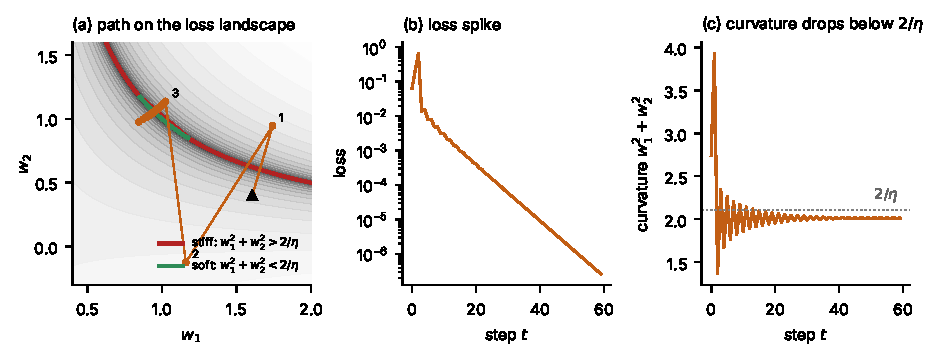
\includegraphics[width=0.62\textwidth]{figs/catapult.pdf}
\caption{A loss spike in two parameters. Gradient descent on $(uv-1)^2/2$ with $\eta=0.95$, started near $(u,v)=(1.6,0.4)$ where the curvature of the valley of minima, $u^2+v^2=2.74$, exceeds $2/\eta=2.11$. (a) The loss jumps from 0.064 to 0.66 and then decays. (b) The curvature oscillates and settles at 2.01, below $2/\eta$.}
\label{fig:catapult}
\end{figure}

\section{Clock 3: generation as a dynamical system}
\label{sec:clock3}

\subsection{Decoding as a stochastic map}

Definition~\ref{def:clock3} makes generation a Markov chain whose state is the whole context. The state space grows with $n$, so the usual results on stationary distributions do not apply directly, but the questions of dynamical systems still make sense: which sets of contexts trap the chain, how long the chain stays in them, and how these answers depend on the temperature $T$ and on truncation. \citet{krishnamurthy2026stochastic} formulate language models as high-dimensional nonlinear autoregressive models and analyze networks of interacting models with mean-field equations. A deterministic version of clock~3, obtained by feeding back the expected embedding of the next-token distribution instead of a sample, is a continuous map that can be analyzed with standard tools \citep{jones2026chaos}.

Temperature divides the logits by $T$, so $\pi_T$ in \eqref{eq:clock3} is a Gibbs distribution with energy $-z$ at temperature $T$. Greedy decoding is the limit $T\to0$, and $T$ sets how often the chain leaves the most likely path, so it serves as both the noise intensity and the natural bifurcation parameter of clock~3. Its effect on task accuracy \citep{renze2024effect} and on novelty and coherence \citep{peeperkorn2024temperature} has been measured directly.

\subsection{Repetition loops as attractors}
\label{sec:loops}

With greedy or low-temperature decoding, models fall into loops that repeat a phrase or sentence until the length limit \citep{holtzman2019curious}. At $T=0$ the chain is deterministic and the loop is one of its periodic orbits. \citet{xu2022learning} showed that loops reinforce themselves: the probability of repeating a sentence grows with the number of times it already appears in the context. Unlikelihood training \citep{welleck2019neural}, truncation rules \citep{hewitt2022truncation,meister2022locally} and feedback control of perplexity \citep{basu2020mirostat} are partly attempts to keep the chain out of these attractors; \citet{fu2020theoretical} give a theoretical analysis of why they form. Recent work studies the inside of the loop: how it shows up in residual-stream dynamics before it becomes visible in the output \citep{zhang2026uncovering}, and the conditions under which a loop ``locks'' so that escape becomes impossible in practice under a given sampler \citep{chen2026repetition}. Loops also appear at the level of whole texts. Repeated paraphrasing converges to period-two attractor cycles even with sampling noise \citep{wang2025unveiling}.

Escape from a loop has the structure of the noise-driven escape problem of Section~\ref{sec:tools}. Suppose the chain has locked into a loop of period $k$ with tokens $a_1,\dots,a_k$. As long as the sampler keeps choosing the loop token, the context is deterministic, so the logits $z_t$ along the loop are fixed numbers. Define the logit gaps $\Delta_t^{j}=z_t(a_t)-z_t(j)$ for $j\neq a_t$; all are positive because the loop is the greedy path. The probability of staying in the loop at step $t$ is
\begin{equation}
p_t(T)=\frac{1}{1+S_t(T)},\qquad S_t(T)=\sum_{j\neq a_t} e^{-\Delta_t^{j}/T},
\label{eq:stay}
\end{equation}
and the probability of leaving during one cycle is $r(T)=1-\prod_{t=1}^{k}p_t(T)$.

\begin{proposition}[Arrhenius law for loop escape]
\label{prop:arrhenius}
Let $\Delta_{\min}=\min_t\min_{j\neq a_t}\Delta_t^{j}$ and let $m$ be the number of pairs $(t,j)$ that attain it. Then $r(T)\le \sum_{t}S_t(T)$ for all $T>0$, and
\begin{equation}
r(T)= m\, e^{-\Delta_{\min}/T}\,\big(1+o(1)\big)\quad\text{as } T\to0,\qquad\text{so}\qquad \lim_{T\to0}T\log r(T)=-\Delta_{\min}.
\end{equation}
\end{proposition}
\begin{proof}
Since $1-\prod_t(1-q_t)\le\sum_t q_t$ for $q_t\in[0,1]$, and $1-p_t=S_t/(1+S_t)\le S_t$, the bound follows. As $T\to0$, each $S_t(T)$ is dominated by its smallest gaps, $S_t(T)=m_t e^{-\delta_t/T}(1+o(1))$ with $\delta_t=\min_j\Delta_t^j$, and $1-\prod_t p_t=\sum_t S_t+O(\max_t S_t^2)$. The terms with $\delta_t=\Delta_{\min}$ dominate the sum.
\end{proof}

The logit gap therefore plays the role of the barrier height $\Delta U$ in Kramers' formula \citep{kramers1940brownian}, and $T$ plays the role of noise intensity. Proposition~\ref{prop:arrhenius} follows almost directly from the Gibbs form of the softmax. The barrier, however, changes with time. Because loops reinforce themselves \citep{xu2022learning}, the gaps grow with each completed cycle, so the well deepens while the chain sits in it. Let $\Delta_c$ be the smallest gap during cycle $c$ and $r_c(T)$ the escape probability during that cycle. The probability of never leaving is $\prod_{c\ge1}(1-r_c(T))$, which is positive exactly when $\sum_c r_c(T)<\infty$ (given $r_c<1$).

\begin{proposition}[Deepening wells lock]
\label{prop:lock}
If $\Delta_c\ge\Delta_1+b\,(c-1)$ for some $b>0$, then for every $T>0$ the probability of never escaping is at least $1-k(|\mathcal V|-1)\,e^{-\Delta_1/T}/(1-e^{-b/T})$ whenever this bound is positive, and it is positive for every $T>0$. If instead the logits along the loop converge from cycle to cycle, so that $\Delta_c\to\Delta_\infty<\infty$, escape eventually happens with probability one, but the expected number of cycles before escape grows like $e^{\Delta_\infty/T}$ as $T\to0$.
\end{proposition}
\begin{proof}
By the bound in Proposition~\ref{prop:arrhenius}, $r_c\le k(|\mathcal V|-1)e^{-\Delta_c/T}$, which is summable under linear growth, and $\prod_c(1-r_c)\ge1-\sum_c r_c$. If the logits converge, then $r_c$ tends to a positive limit and the second statement follows from the first part of Proposition~\ref{prop:arrhenius}.
\end{proof}

In practice logits are bounded, so the gaps must saturate and the second case applies; ``locking'' then means that the escape time exceeds any realistic generation budget. Experiment~3 (Section~\ref{sec:exp3}) measures $\Delta_c$ along real loops of GPT-2 and tests both propositions against the exact survival probabilities and against Monte Carlo sampling.

\subsection{Temperature-driven transitions}

At the level of statistics over many generations, temperature produces something close to a phase transition. \citet{nakaishi2024phase} varied $T$ in GPT-2 and found a low-temperature phase with repetitive structure, a high-temperature phase of incoherent text, and power-law correlations close to those of natural language at the transition point. \citet{arnold2024phase} proposed statistical methods to detect such transitions automatically from output distributions. \citet{jones2026chaos} found that in the continuous feedback version of generation, temperature and activation steering move the system between periodic orbits and chaos with positive finite-time Lyapunov exponents, with period-doubling scaling and periodic orbits proved by interval arithmetic. In chain-of-thought trajectories, \citet{jaca2026chaos} report sensitive dependence on initial conditions together with bounded evolution and fractal structure in hidden-state space. Sorting many generated trajectories into regimes (fixed point, periodic, irregular) without labels is a response-regime identification problem, for which unsupervised data-driven methods exist in mechanics \citep{farid2024unsupervised}.

\subsection{Drift over long horizons}

Training uses teacher forcing, while generation feeds the model its own outputs. Small errors therefore compound along clock~3, a problem known as exposure bias \citep{bengio2015scheduled,wang2020exposure}. Errors snowball in multi-step reasoning \citep{dziri2023faith} and in hallucinated justifications \citep{zhang2023language}, and next-token prediction can fail on planning tasks that require looking ahead \citep{bachmann2024pitfalls}. In dynamical terms these are statements about the growth of perturbations along a trajectory of the closed-loop system, which is what Lyapunov exponents measure.

\subsection{Outer loops: when generation feeds training}

The slow-fast separation of Section~\ref{sec:maps} breaks when generated text is used for training. Training repeatedly on a model's own outputs makes the tails of the distribution disappear \citep{shumailov2023curse,alemohammad2023selfconsuming}; whether the process stays near the original model depends on the fraction of real data in each round \citep{bertrand2023stability}. Reinforcement learning from human feedback reduces output diversity \citep{kirk2023effects}, which can be read as a contraction of the set of trajectories that clock~3 visits. These are dynamical systems over model versions, a fourth and much slower clock.

\subsection{Language models as models of dynamical systems}

A different line of work asks whether language models can forecast dynamical systems placed in their context. Pretrained models forecast time series zero-shot \citep{gruver2023large} and extrapolate trajectories of physical systems with accuracy that improves with context length \citep{liu2024llms}. Chaotic systems serve as a benchmark for such forecasters \citep{gilpin2021chaos,gilpin2023model,pathak2018model}, and training on data from cellular automata at the edge of chaos produces models with better downstream reasoning \citep{zhang2024intelligence}. These results are about the content a model processes, not about the model as a dynamical system, but they share tools with this paper.

\section{The Three-Clock Dictionary}
\label{sec:dictionary}

Table~\ref{tab:dictionary} collects the results of Sections~\ref{sec:clock1}, \ref{sec:clock2} and~\ref{sec:clock3}. Each row is a concept from nonlinear dynamics and each column is a clock. A cell names the observed behavior that the concept describes on that clock and marks its evidence level: \statusP\ when the correspondence is proved for a model of the system, \statusM\ when it has been measured in trained networks, and \statusC\ when it is a conjecture. A question mark means that we found no work that tests the concept on that clock.

\begin{table}[p]
\centering
\scriptsize
\setlength{\tabcolsep}{3pt}
\renewcommand{\arraystretch}{1.25}
\begin{tabularx}{\textwidth}{>{\raggedright\arraybackslash}p{2.1cm} >{\raggedright\arraybackslash}X >{\raggedright\arraybackslash}X >{\raggedright\arraybackslash}X}
\toprule
\textbf{Concept} & \textbf{Clock 1: layer time $\ell$} & \textbf{Clock 2: training time $t$} & \textbf{Clock 3: generation time $n$} \\
\midrule
Fixed point & Tokens collapse to a cluster; rank collapse \statusP\ \citep{geshkovski2023mathematical,dong2021attention}. Massive activations nearly input independent \statusM\ \citep{sun2024massive} & Convergence to a minimum; neural collapse at the end of training \statusM\ \citep{papyan2020prevalence} & Period-one loops (one token repeated) as the simplest case of degenerate repetition \statusM\ \citep{holtzman2019curious} \\
Linear stability, Jacobian spectrum & Dynamical isometry; layer Jacobians of trained models \statusP/\statusM\ \citep{pennington2017resurrecting,fernando2026dynamics} & Sharpness vs.\ $2/\eta$ \statusM\ \citep{cohen2021gradient} & Derivative of the feedback map factorizes through $1/T$ \statusM\ \citep{jones2026chaos} \\
Finite-time Lyapunov exponent & Ridges in input space separate classes \statusM\ \citep{storm2023finitetime}; per-layer profile over training \statusM\ (Sec.~\ref{sec:exp1}) & Sensitivity of runs to minibatch noise early in training \statusM\ \citep{frankle2019linear} & Divergence of nearby generations \statusM\ \citep{jaca2026chaos,jones2026chaos} \\
Edge of chaos, criticality & Order-chaos transition at initialization sets trainable depth \statusP\ \citep{poole2016exponential,schoenholz2016deep} & Edge of stability \statusM\ \citep{cohen2021gradient} & Critical temperature with power-law text statistics \statusM\ \citep{nakaishi2024phase} \\
Limit cycle (periodic orbit) & \na & Period-2 orbits of GD \statusP\ \citep{chen2022edge}; SGD converges to cycles \statusP\ \citep{chaudhari2017stochastic} & Repetition loops \statusM\ \citep{xu2022learning}; paraphrase 2-cycles \statusM\ \citep{wang2025unveiling}; loops converge in hidden-state space \statusM\ (Exp.~3) \\
Period doubling, route to chaos & \na & Larger step sizes give period doubling and chaos in minimal models \statusP\ \citep{zhu2022edgeofstability,kong2020stochasticity}; period-2 orbit, then irregular oscillation, in a transformer \statusM\ (Exp.~2) & Feigenbaum scaling in embedding feedback \statusM\ \citep{jones2026chaos} \\
Fractal boundary & \na & Trainable vs.\ divergent hyperparameters \statusM\ \citep{sohldickstein2024boundary}; interleaved trainable and divergent step sizes \statusM\ (Exp.~2); fractal attractors of optimizers \statusM\ \citep{tuci2026generalization} & \na \\
Basin of attraction & Class regions bounded by FTLE ridges \statusM\ \citep{storm2023finitetime} & Which minimum is reached depends on step size and batch size \statusM\ \citep{jastrzebski2017three} & Prompts that do or do not fall into loops \statusC \\
Metastability, slow manifold & Multi-cluster states last exponentially long \statusP\ \citep{geshkovski2024dynamic} & Plateaus \statusP\ \citep{saxe2013exact}; slow phase of pretraining \statusM\ \citep{zhang2026stability,wen2024warmupstabledecay} & Long coherent stretches before drift \statusC \\
Saddle and ghost & \na & Saddles dominate \statusM\ \citep{dauphin2014identifying}; abrupt learning from a ghost \statusP\ \citep{dinc2025ghost} & \na \\
Phase transition & \na & Grokking \statusP/\statusM\ \citep{rubin2023grokking,power2022grokking}; induction heads \statusM\ \citep{olsson2022incontext} & Low-$T$ repetitive vs.\ high-$T$ incoherent phase \statusM\ \citep{nakaishi2024phase,arnold2024phase}; narrow coherent window between them, also in a reasoning model \statusM\ (Exp.~3) \\
Noise-driven (Kramers) escape & \na & Escape of SGD from minima \statusP\ \citep{xie2020diffusion,mori2021powerlaw} & Escape from repetition loops, logit gap as barrier \statusP/\statusM\ (Prop.~\ref{prop:arrhenius}, Exp.~3); locking temperature \statusP\ (Prop.~\ref{prop:tlock}), horizon-dependent in practice \statusM\ (Exp.~3) \\
Synchronization, consensus & Clustering as consensus; Kuramoto form \statusP\ \citep{geshkovski2023mathematical,li2026diverse}; synchronization by noise \statusP\ \citep{agazzi2026stochastic} & \na & Collective dynamics of interacting models \statusP\ \citep{krishnamurthy2026stochastic} \\
Koopman, linearization & Local linear description of each layer \statusM\ \citep{fernando2026dynamics} & Koopman-based training and pruning \statusM\ \citep{dogra2020optimizing,redman2021operator}; lazy regime \statusP\ \citep{jacot2018neural} & \na \\
Conservation law, symmetry & Gradient-flow structure of attention \statusP\ \citep{sander2021sinkformers} & Symmetries give conserved quantities that finite steps break \statusP\ \citep{kunin2020neural} & \na \\
\bottomrule
\end{tabularx}
\caption{The Three-Clock Dictionary. Each cell gives the behavior that a dynamical-systems concept describes on one clock, with its evidence level (\statusP: proved in a model; \statusM: measured in trained networks; \statusC: conjecture) and representative references. Question marks are cells for which we found no study; they define the open problems of Section~\ref{sec:open}.}
\label{tab:dictionary}
\end{table}

\paragraph{Reading the table by rows.} Fixed points, stability and Lyapunov exponents have been used on all three clocks, although with different meanings: on clock~1 they describe a single finite trajectory, on clock~2 the long-run behavior of an optimizer, and on clock~3 a random process. Phase transitions and escape appear on clocks~2 and~3 but not on clock~1, where the number of steps is fixed and small, so there is no long-time limit in which a transition could be sharp. Even so, the metastability result of \citet{geshkovski2024dynamic} shows that finite-time transients on clock~1 can be analyzed with care.

\paragraph{Reading the table by columns.} Clock~2 is the best covered column, because optimization theory has always been a theory of iterated maps. Clock~1 is covered mostly by results at initialization and by models with simplified attention. Clock~3 is the youngest column, and most of its entries date from 2024 or later.

\paragraph{Where the analogies are weak.} First, clock~1 runs for a fixed and small number of steps (between 6 and about 100 layers), so asymptotic notions such as attractors and Lyapunov exponents must be replaced by finite-time versions. Second, clock~2 is driven by a data stream whose statistics are not stationary in general, and by learning-rate schedules, which makes it a non-autonomous system. Third, the state of clock~3 is the whole context, so its dimension grows with time and the chain never returns to an earlier state. Statements about loops and attractors on clock~3 are therefore about the projection of the state onto recent tokens. Each of these differences limits which theorems can be imported from the classical theory without change.

\section{Three experiments, one per clock}
\label{sec:experiments}

Each experiment below takes one concept from Table~\ref{tab:dictionary}, measures it on open models, and runs on a two-core CPU in under two hours. Details are in Appendix~\ref{app:details}, and the code reproduces every number.

\subsection{Experiment 1: the Lyapunov profile of the residual stream over training (clocks 1 and 2)}
\label{sec:exp1}

\paragraph{Question and setup.} Finite-time Lyapunov exponents \eqref{eq:ftle} describe how a forward pass stretches perturbations, layer by layer. How does this profile change as the model trains? This question couples clock~1 to clock~2 (\op{1}). We use the public training checkpoints of Pythia \citep{biderman2023pythia}: eleven checkpoints of Pythia-70M (6 layers), from initialization to step 143{,}000, and six checkpoints of Pythia-160M (12 layers). Each block is treated as a map $F_\ell$ on the full residual stream of a 16-token context. For each block we estimate the largest singular value $\sigma_\ell$ of its Jacobian by power iteration and report the relative exponent
\begin{equation}
\tilde\Lambda_\ell=\log\sigma_\ell-\log\big(\|x^{\ell+1}\|/\|x^{\ell}\|\big),
\end{equation}
which measures stretching beyond the growth of the residual norm. For the whole stack we report $\Lambda=\frac{1}{L}\log\sigma_{\max}(\mathrm{D}F_{0\to L})$, and the ratio $\kappa=\log\sigma_{\max}(\mathrm{D}F_{0\to L})/\sum_\ell\log\sigma_\ell$. Since $\sigma_{\max}$ of a product is at most the product of the $\sigma_\ell$, $\kappa\le1$ whenever $\sum_\ell\log\sigma_\ell>0$, which holds throughout our measurements, and $\kappa$ near one means that the most expanded direction of each layer is passed on to the next. Values are means over eight prompts, and $\kappa$ is the ratio of the two means.

\paragraph{Results.} Figure~\ref{fig:exp1} shows three things. First, at initialization both models have the same profile, decreasing with depth ($\tilde\Lambda_\ell$ from 1.20 to 0.53 in Pythia-70M and from 1.19 to 0.39 in Pythia-160M), which reflects the shared initialization scheme. Second, training makes every layer more expansive. The mean of $\tilde\Lambda_\ell$ over layers rises from 0.75 to 2.32 in Pythia-70M and from 0.59 to 2.17 in Pythia-160M, and it is still rising at the last checkpoint. The rise is not monotone at first: at step 128 the deepest layers of Pythia-70M contract further (layer 6 drops from 0.53 to 0.22) before all layers expand. Third, the whole stack does not follow. In Pythia-70M, $\Lambda$ goes from 0.87 to about 1.1 and stays between 1.11 and 1.18 from step 4{,}000 onward, which is under 3\% of training. In Pythia-160M it moves from 0.45 to 0.58. As a result the coherence $\kappa$ falls during training, from 0.67 to 0.36 in Pythia-70M and from 0.52 to 0.22 in Pythia-160M.

\paragraph{Reading.} Training produces layers that are individually more sensitive to perturbations, while the expanding directions of consecutive layers become less aligned, so the forward pass as a whole stretches perturbations only moderately. The depth-averaged exponent settles early, while the per-layer exponents keep changing. This is consistent with the observation that the normalized singular value spectra of the weights stabilize early in pretraining \citep{zhang2026stability}, now seen through the Jacobians of the forward map. These are measurements on two small models with short contexts and a small prompt set. Whether the same pattern holds at scale, and whether $\kappa$ predicts robustness to perturbations or the success of model editing, is part of \op{1}.

\begin{figure}[t]
\centering
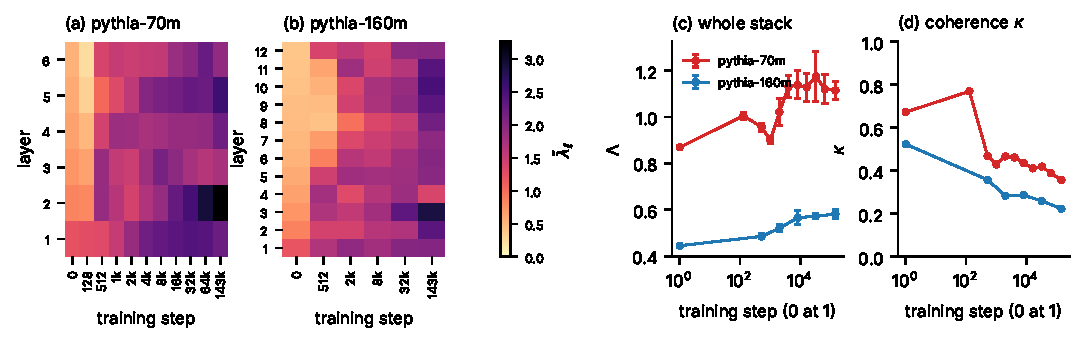
\includegraphics[width=\textwidth]{figs/exp1_ftle.pdf}
\caption{Experiment 1: finite-time Lyapunov exponents of the residual stream across public Pythia checkpoints. (a, b) Relative per-layer exponent $\tilde\Lambda_\ell$ (stretching of the top singular direction beyond the growth of the residual norm) for each layer and checkpoint. (c) Depth-averaged exponent of the whole stack, $\Lambda$; bars: standard deviation over prompts. (d) Coherence $\kappa$ between per-layer and whole-stack stretching; values below one mean that the most expanded directions of consecutive layers are not aligned.}
\label{fig:exp1}
\end{figure}


\subsection{Experiment 2: a learning-rate bifurcation diagram (clock 2)}
\label{sec:exp2}

\paragraph{Question and setup.} How does the long-run behavior of gradient descent on a transformer change with the step size $\eta$? We train a one-block transformer (two heads, width 32) with full-batch gradient descent on next-token prediction of sequences from a fixed random Markov chain, for 56 step sizes between $0.02$ and $4$. Within one seed every step size starts from the same initialization and sees the same data, and we repeat the sweep for three seeds that change both. Full batches remove minibatch noise, so any irregularity comes from the map \eqref{eq:clock2} itself. For each run we record the last 400 losses and the sharpness $\lambda_{\max}$ at the end.

\paragraph{Results.} Figure~\ref{fig:exp2} shows three regimes. In each seed, 48 of the 56 step sizes train. Across these 144 runs the final sharpness sits just above the stability threshold, with $\eta\lambda_{\max}/2$ having median $1.07$ and range $[1.00,1.21]$ across two decades of step size (panel b). This is the edge-of-stability behavior of \citet{cohen2021gradient}, and in this model it holds over the entire trainable range we tested. None of the runs settles on a fixed point. Removing the slow downward trend of the loss shows what the iterate does instead (panels a and c). For $\eta<0.05$ the fluctuations alternate in sign at every step, a period-2 orbit riding on the slow descent, and the median lag-1 autocorrelation of the detrended loss over the ten smallest step sizes is $-0.99$, $-0.99$ and $-0.97$ in the three seeds. As $\eta$ grows the fluctuations become larger and less regular. The median lag-1 autocorrelation rises to between $-0.95$ and $-0.92$ for $0.05\le\eta<0.3$, between $-0.74$ and $-0.68$ for $0.3\le\eta<1$, and between $-0.66$ and $-0.32$ for $\eta\ge1$. The edge of trainability depends on the seed. In seed 0 every $\eta\ge2.04$ diverges, while in seeds 1 and 2 divergent and trainable step sizes interleave between $1.5$ and $2.5$, and in seed 1 the largest trainable step size (2.47) lies above the smallest divergent one (1.68).

\paragraph{Reading.} In dictionary terms, the trainable range of this model is a sequence from a period-2 orbit near the stability boundary, through increasingly irregular oscillation, to divergence. This is the picture that minimal models predict \citep{chen2022edge,zhu2022edgeofstability,kong2020stochasticity}, here measured on a transformer with attention and layer normalization. The interleaving of trainable and divergent step sizes near the edge is consistent with the fractal trainability boundary reported by \citet{sohldickstein2024boundary}, although a grid of 56 points cannot measure a fractal dimension. We do not claim a full period-doubling cascade, since with 400-step tails on top of a slowly drifting loss we cannot resolve periods above two.

\begin{figure}[t]
\centering
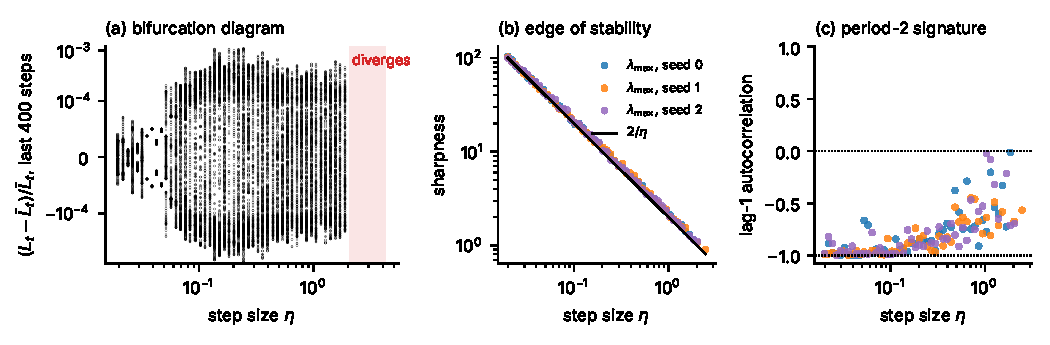
\includegraphics[width=\textwidth]{figs/exp2_bifurcation.pdf}
\caption{Experiment 2: full-batch gradient descent on a one-block transformer. (a) Bifurcation diagram for seed 0: relative deviation of the last 400 losses from their running mean (9-step window, symmetric-log axis) against the step size. Two branches at small $\eta$ mark a period-2 orbit; the band at larger $\eta$ is irregular oscillation; the shaded region diverges. (b) Sharpness at the end of training against $2/\eta$ for three seeds. (c) Lag-1 autocorrelation of the detrended loss for the same runs; $-1$ is a clean period-2 orbit.}
\label{fig:exp2}
\end{figure}

\subsection{Experiment 3: escape from repetition loops (clock 3)}
\label{sec:exp3}

\paragraph{Question and setup.} Section~\ref{sec:loops} predicts that escape from a repetition loop follows an Arrhenius law with the logit gap as barrier (Proposition~\ref{prop:arrhenius}), and that loops lock if the barrier grows from cycle to cycle (Proposition~\ref{prop:lock}). We test both on GPT-2 small \citep{radford2019language} and on the final checkpoint of Pythia-160M \citep{biderman2023pythia}. From each of 40 prompts we decode greedily for 320 tokens and keep the runs that end in a loop. Because the context along a loop is deterministic, the logits stored during the greedy run give the exact probability of staying in the loop at any temperature, and we check these exact values against Monte Carlo sampling.

\paragraph{Results.} Greedy decoding ends in a loop for 37 of the 40 prompts in each model, with periods from 4 to 53 tokens (median 23) in GPT-2 and from 7 to 46 tokens (median 22) in Pythia-160M (Figure~\ref{fig:exp3}).

The barrier grows. The median smallest logit gap $\Delta_c$ rises from 0.36 in the second cycle of a loop to 2.33 in the sixth and 3.63 in the twentieth in GPT-2, and from 0.47 to 1.83 and then 2.77 by the tenth cycle in Pythia-160M (panel a). The barrier in cycle 6 is larger than in cycle 2 for 36 of 36 GPT-2 loops and 35 of 37 Pythia-160M loops. This is the self-reinforcement reported by \citet{xu2022learning}, measured here as the depth of a well.

Escape follows the Arrhenius law. For the first cycle after two cycles of burn-in, the escape probability per cycle approaches $e^{-\Delta_{\min}/T}$ at low temperature (panel b). Fitting $\log r$ against $1/T$ recovers the measured barrier with a correlation of 0.997 in both models and a median relative difference of 6.9\% (22 GPT-2 loops) and 5.7\% (21 Pythia-160M loops). Loops whose escape probability never falls below $10^{-2}$ on our temperature grid are excluded from the fit (panel c). The exact survival probabilities agree with Monte Carlo sampling. Across 24 comparisons per model (four loops, two temperatures, survival after 1, 2 and 4 cycles, 128 samples each), the largest absolute difference is 0.062 for GPT-2 and 0.068 for Pythia-160M, and every difference is within two binomial standard errors.

Loops lock below a fairly sharp temperature. The median probability of staying in a loop until the end of the 320-token horizon is 0.89 at $T=0.31$ in both models, crosses 0.5 at $T\approx0.53$ (GPT-2) and $T\approx0.48$ (Pythia-160M), and falls to 0.06 and 0.015 at $T=0.75$ (panel d). Free sampling gives a consistent picture. After 200 tokens, 80\% (GPT-2) and 82.5\% (Pythia-160M) of generations end in a loop at $T=0.3$, 50\% and 35\% at $T=0.5$, at most 7.5\% at $T=0.7$, and none at $T\ge0.85$.

\paragraph{Reading.} The escape problem on clock~3 has the structure of Kramers' problem, with two differences that matter. The noise acts on a discrete choice through a Gibbs distribution, so the Arrhenius form follows directly from the softmax (Proposition~\ref{prop:arrhenius}) and needs no diffusion approximation. In addition, the barrier is a function of the residence time, so a loop becomes harder to leave the longer the model repeats it. Panel (a) also shows that the deepening is not uniform, and barriers often rise quickly over the first five cycles, pause, and rise again. Escape from a well whose depth grows with the time already spent in it is a non-stationary escape problem. Its mechanical analogue is a particle in a well that deepens as the particle settles, and its scaling with model size is open (\op{5}).

\begin{figure}[t]
\centering
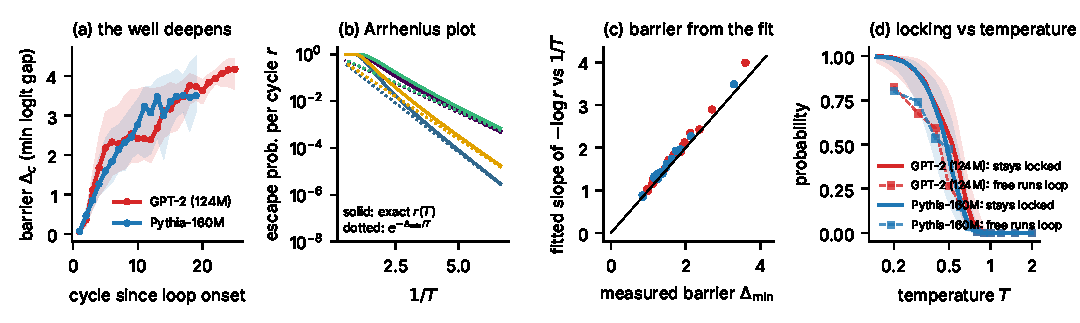
\includegraphics[width=\textwidth]{figs/exp3_escape.pdf}
\caption{Experiment 3: escape from repetition loops. (a) Barrier $\Delta_c$ (smallest logit gap in cycle $c$) against cycles since loop onset; line: median over loops, band: interquartile range; only cycles reached by at least 10 loops are shown. (b) Exact escape probability per cycle for four GPT-2 loops (solid) and the Arrhenius term $e^{-\Delta_{\min}/T}$ (dotted). (c) Barrier recovered from the slope of $\log r$ against $1/T$ at low temperature, against the measured $\Delta_{\min}$; line: identity. (d) Solid: median probability of staying in the loop until the end of the 320-token horizon, after two cycles of burn-in (band: interquartile range); the number of remaining cycles differs between loops because their onsets differ. Dashed: fraction of free generations of 200 tokens that end in a loop.}
\label{fig:exp3}
\end{figure}

\FloatBarrier
\section{Open problems}
\label{sec:open}

The experiments answered some questions and opened others. Each problem below comes from an empty or weak cell of Table~\ref{tab:dictionary}, from a result of Section~\ref{sec:experiments}, or from a place where two clocks meet, and each is stated with a first test. Problems \op{9} and \op{10} are conjectures that come from the mechanics of nonlinear oscillators; we include them because they make predictions that can be checked, and we do not claim evidence for them yet.

\begin{enumerate}[label=\textbf{OP\,\arabic*.}, leftmargin=*, itemsep=3pt]
\item \textbf{Coupling of clocks 1 and 2.} Which features of the Lyapunov profile of the forward pass settle before the loss does? In two small models the whole-stack exponent settles within 3\% of training while the per-layer exponents keep growing (Experiment~1). The next test is the full Jacobian spectrum of every layer across the public checkpoints of a model family above a billion parameters.

\item \textbf{Periodic orbits in depth.} Do models that reuse a block many times, such as looped and recurrent-depth models \citep{prairie2026parcae}, have periodic or quasi-periodic orbits in the residual stream, and do these orbits carry computation? Return maps of hidden states over many loop iterations would show them directly.

\item \textbf{The full Lyapunov spectrum of a language model.} How many directions expand along a forward pass and along a generation, and what is the resulting attractor dimension? QR-based algorithms \citep{engelken2020lyapunov,vogt2020lyapunov} make this feasible for models of GPT-2 size, and the exponent of clock~3 would turn exposure bias into a measured quantity.

\item \textbf{The type of a loss spike.} Are the loss spikes of pretraining crossings of the stability boundary, period-doubling cascades, catapults \citep{lewkowycz2020large} or escapes from a basin? Each type leaves a different signature in the curvature and in the update direction just before the spike, so open training logs and checkpoints can be classified by these signatures.

\item \textbf{Escape laws across samplers and scales.} How do nucleus sampling and repetition penalties change the barrier of Proposition~\ref{prop:arrhenius}, and do the saturated barrier and the locking temperature keep growing with model size beyond 1B parameters? Reasoning models add the recurrent orbits of Experiment~3, which have no period: do they have an escape law of their own, and do recurrence plots of the trace predict when a model will run out of budget? A harder version asks whether the onset of a loop and the coherent window of a prompt can be read from the prompt and the weights before any text is generated.

\item \textbf{Fractal trainability of transformers.} Does the fractal boundary between convergent and divergent hyperparameters \citep{sohldickstein2024boundary}, reproduced for a small network in Figure~\ref{fig:basins}, persist for transformers trained with Adam, and how does its dimension depend on depth? Fine grids over learning rate and warmup length give a first estimate.

\item \textbf{Metastability in generation.} Is the length of a coherent stretch of generated text before drift a metastable residence time, exponentially long in some barrier, like the cluster states in depth \citep{geshkovski2024dynamic}? Survival curves of coherence against temperature would test this.

\item \textbf{Koopman modes of a forward pass.} Can a linear operator fitted to residual-stream trajectories predict the effect of an intervention several layers ahead, and do its eigenfunctions align with known features? Dynamic mode decomposition on residual streams, compared with the tuned lens \citep{belrose2023eliciting}, is a direct test.

\item \textbf{Targeted energy transfer (conjecture).} In coupled mechanical oscillators, a nonlinear energy sink absorbs vibration energy from a primary system in one direction and irreversibly \citep{vakakis2009nonlinear,farid2016tuned}. We conjecture a similar one-way transfer of signal energy between spectral modes of the residual stream, with massive activations and attention sinks \citep{sun2024massive,xiao2023efficient} in the role of the sink. Tracking the energy of each singular mode of the layer Jacobians across depth and training would confirm or refute it.

\item \textbf{Escape under internal forcing (conjecture).} At the edge of stability the iterate oscillates along stiff directions, and the other directions see this oscillation as periodic forcing. A periodically forced particle escapes from a potential well when the forcing amplitude crosses a threshold that depends on the forcing frequency \citep{farid2019escape,farid2022escape}, and we conjecture that some loss spikes are escapes of this kind. Gradient descent on a quartic well coupled to an oscillating direction is the simplest test. Experiment~2 adds a related question: self-stabilization \citep{damian2022selfstabilization} explains a single mode at the edge, but our transformer has several, which exchange order at every step, and their averaged dynamics is open.

\item \textbf{Early warning signals.} Near a bifurcation, recovery from perturbations slows down and fluctuations grow. Do grokking, induction-head formation and loss spikes show rising autocorrelation and variance of the loss or of the gradient norm before they happen? Runs with a known transition step \citep{power2022grokking,olsson2022incontext} allow a direct check.

\item \textbf{Control of clock 3.} Can a controller built from the escape analysis keep generation coherent at a lower cost than repetition penalties, with Mirostat \citep{basu2020mirostat} and truncation sampling \citep{hewitt2022truncation} as baselines? Three first tests on GPT-2 (Appendix~\ref{app:exp3}) fail in an instructive way. Heating the sampler when a loop is detected cuts looping generations at $T=0.3$ from 68\% to 6\%, but 94\% of the outputs remain repetitive. Rolling the text back to the first token of a loop and resampling there removes all exact loops at $T=0.5$, but 91\% of the outputs stay repetitive. A feedback controller on recurrence and surprisal settles near the center of the coherent window from any start, but its share of coherent texts (21\% to 83\%) does not beat the 82\% of the best fixed temperature. All three act on the noise, while the trap is stored in the context. Controllers that act on the state, by editing the cache or by adding a steering vector to the residual stream \citep{turner2023steering,zou2023representation}, are the natural next step: in mechanical terms, a control force on the state instead of a change of the noise intensity.
\end{enumerate}

\section{Conclusion}
\label{sec:conclusion}

A transformer language model is iterated in three ways: over layers, over optimizer steps and over generated tokens. Each iteration has been studied with tools from dynamical systems, mostly by different communities and under different names. We gave the three iterations one formal frame, reviewed the results on each, and summarized them in a dictionary that records which concepts have been proved, measured or only conjectured on which clock. In experiments on open models we found that training makes each layer of a Pythia model more expansive while the coherence of the whole forward pass falls, and that gradient descent on a small transformer stays at a multi-mode edge of stability across two decades of step size. Repetition loops in GPT-2 and Pythia behave as wells whose depth grows while the model sits in them and then saturates. Whether a loop locks therefore depends on the length of the generation and on the size of the model, and coherent text lies in a narrow temperature window between repetition and incoherence. A small reasoning model has the same window, centered on its recommended temperature, and its low-temperature failure is recurrent rethinking, with no periodic loop.

A bridge between two fields can describe, explain and solve. This paper describes the three clocks in one vocabulary, shows the correspondences side by side, derives the reduced-order models behind them, and explains several behaviors that the machine learning literature had measured but not accounted for, from the Arrhenius escape from loops to the narrow window of coherent text. It does not yet solve a problem of language models that was unsolved before: our controllers for repetition find the right temperature but do not beat it. We think the third level is within reach, because many problems of language models have counterparts that dynamics has already solved, and the open problems of Section~\ref{sec:open} point to where.

Many cells of the dictionary are empty, and several of the open problems sit where two clocks meet, such as the effect of training on the depth dynamics, the feedback of generated text into training, and the prediction of training instabilities with the tools used for escape problems in mechanics. Each of these questions has a counterpart that nonlinear dynamics has studied for decades on pendulums, ships and oscillator networks, and each can be tested with the weights and outputs of open models on a laptop. We hope that the shared vocabulary of this paper helps researchers from both communities recognize the same phenomenon when they meet it, and solve it together.

\subsubsection*{Code and data}
Code to reproduce every figure and number, the raw results, and a maintained list of the papers in this review are available \codeurl. All experiments run on a CPU.

\subsubsection*{Broader impact statement}
This is a review with small-scale experiments on public models, and we do not foresee direct negative consequences. A better account of repetition loops and of training instabilities could reduce wasted compute in pretraining and make generation more reliable.

\subsubsection*{Use of AI tools}
\label{sec:ai}
An AI assistant (Claude, Anthropic) was used to search and verify the literature, draft and edit text, and write and run experiment code under the author's direction. All references were checked against arXiv or Crossref records, all numbers come from the released code, and the author is responsible for every claim in the paper.


\bibliography{refs}
\bibliographystyle{tmlr}

\appendix
\section{Experimental details}
\label{app:details}

All experiments run on a CPU with two cores and 7\,GB of memory, using PyTorch and Hugging Face Transformers with the public checkpoints of GPT-2 small \citep{radford2019language} and Pythia \citep{biderman2023pythia}. The repository contains one script per experiment, the exact command lines, the raw JSON outputs and the plotting scripts. The 40 prompts used in Experiments~1 and~3 are short neutral sentence openings written for this study (for example, ``The weather today is cold and cloudy, with a chance of''), and the full list is in the repository.

\subsection{Experiment 1: finite-time Lyapunov exponents}
\label{app:exp1}

For each prompt we take the first $T$ tokens (prompts shorter than $T$ are repeated) and run the model once to record the residual stream $x^0,\dots,x^L$ before the final layer normalization. We then call each block of the Hugging Face implementation directly as a function $F_\ell:\mathbb{R}^{T\times d}\to\mathbb{R}^{T\times d}$, with rotary embeddings and an explicit causal mask, and check that chaining these calls reproduces the model's hidden states (the maximum relative deviation was zero in float32 for every checkpoint). The largest singular value of the Jacobian $DF_\ell(x^\ell)$ is estimated by power iteration on $DF_\ell^{\top}DF_\ell$, using forward-mode (JVP) and reverse-mode (VJP) products from \texttt{torch.func}. The same procedure applied to the composition $F_{L-1}\circ\cdots\circ F_0$ gives the depth-averaged exponent $\frac{1}{L}\log\sigma_{\max}(DF_{0\to L})$. We use eight prompts, contexts of 16 tokens and 10 power iterations per estimate, for eleven Pythia-70M checkpoints (steps 0, 128, 512, 1k, 2k, 4k, 8k, 16k, 32k, 64k and 143k) and six Pythia-160M checkpoints (steps 0, 512, 2k, 8k, 32k and 143k).

\subsection{Experiment 2: bifurcation diagram}
\label{app:exp2}

\emph{Data.} A first-order Markov chain over $V=12$ symbols, with transition rows drawn from a Dirichlet distribution with concentration $0.3$ (seed 0), generates $N=64$ sequences of length 13, and the model predicts the next symbol at each of the 12 positions. \emph{Model.} One pre-LN transformer block with causal attention (two heads, width 32, MLP width 64), learned positional embeddings and a linear readout, in float64. Attention is written out explicitly so that Hessian-vector products work on a CPU. \emph{Training.} Full-batch gradient descent on the mean cross-entropy, from the same initialization for every step size within a seed. Seeds 0, 1 and 2 change both the Markov chain and the initialization. Each run lasts $\max(3000,\,600/\eta)$ steps, capped at 30{,}000, so that all runs cover a comparable amount of gradient-flow time. A run is marked as diverged if the loss exceeds 50 or becomes non-finite. \emph{Measurements.} The last 400 losses of each run, and the top Hessian eigenvalue at the final iterate from 40 steps of power iteration on Hessian-vector products. The step sizes are 56 values spaced geometrically between $0.02$ and $4$.

\subsection{Experiment 3: escape from repetition loops}
\label{app:exp3}

\emph{Loop detection.} From each prompt we decode greedily for 320 tokens and store the full logit vector at each step. A loop of period $k\le64$ is detected when the last $3k$ tokens are $k$-periodic, and its onset is the earliest index from which the sequence stays $k$-periodic. \emph{Stay probabilities.} Along the loop the context is deterministic, so the probability \eqref{eq:stay} of producing the loop token at temperature $T$ follows from the stored logits, for 30 temperatures spaced geometrically between $0.15$ and $2$. From these we compute, for each cycle $c$, the barrier $\Delta_c$ (smallest gap between the loop token's logit and any other logit during the cycle) and the escape probability $r_c(T)=1-\prod_{t\in c}p_t(T)$. \emph{Arrhenius fit.} For the first cycle after two completed cycles of burn-in, we fit $\log r$ against $1/T$ by least squares over the temperatures where $10^{-9}<r<10^{-2}$, and compare the negative slope with $\Delta_{\min}$ of that cycle. \emph{Monte Carlo check.} For the first four loops we sample 128 continuations at $T\in\{0.6,1.0\}$ (nearest grid temperature) from the context after burn-in, record the first step whose token differs from the loop, and compare the fraction still in the loop after 1, 2 and 4 cycles with the exact survival probability. \emph{Free sampling.} For each of seven temperatures we sample 200 tokens from every prompt with plain temperature sampling (no top-$k$ or top-$p$) and record whether the output ends in a loop with at least three repetitions.


\end{document}
